\documentclass[pdflatex,sn-nature]{sn-jnl}

\usepackage{graphicx}
\usepackage{manyfoot}
\usepackage{amsmath,amssymb,amsfonts}
\usepackage{booktabs}
\usepackage{longtable}
\usepackage{multirow}
\usepackage{array}
\usepackage{tabularx}
\usepackage{url}
\usepackage{xcolor}
\usepackage[section]{placeins}

% sn-jnl loads article in twoside mode; disable alternating odd/even margins
% so the compiled PDF has a stable text block in Overleaf and exported previews.
\makeatletter
\@twosidefalse
\@mparswitchfalse
\makeatother

\raggedbottom

\begin{document}

\title[TIMELY Bench]{TIMELY Bench for Temporal Clinical Reasoning in Critical Care}

\author*[1]{\fnm{Haoyu} \sur{Wang}}\email{haoyu.7.wang@kcl.ac.uk}
\equalcont{These authors contributed equally: Haoyu Wang, Zitong Li, Linglong Qian, and Zina Ibrahim.}

\author[1]{\fnm{Zitong} \sur{Li}}\email{zitong.2.li@kcl.ac.uk}
\equalcont{These authors contributed equally: Haoyu Wang, Zitong Li, Linglong Qian, and Zina Ibrahim.}

\author[1]{\fnm{Linglong} \sur{Qian}}\email{linglong.qian@kcl.ac.uk}
\equalcont{These authors contributed equally: Haoyu Wang, Zitong Li, Linglong Qian, and Zina Ibrahim.}

\author[1]{\fnm{Zina} \sur{Ibrahim}}\email{zina.ibrahim@kcl.ac.uk}
\equalcont{These authors contributed equally: Haoyu Wang, Zitong Li, Linglong Qian, and Zina Ibrahim.}

\affil*[1]{\orgname{King's College London}, \orgaddress{\city{London}, \country{United Kingdom}}}

\abstract{Temporal clinical reasoning requires interpreting partially observed patient trajectories, yet most clinical AI benchmarks test static prediction, medical question answering, or workflow execution. Using MIMIC-IV ICU stays, we developed TIMELY Bench, an ICU benchmark aligning AKI, delirium, sepsis, and stroke on a 168-hour hourly grid with anchor-bounded multimodal EHR prompts spanning structured measurements, medications, procedures, clinical notes, and condition-specific observations. The frozen evaluation sample included 12,000 instances from 9,587 ICU stays, expanded to 53,070 \texttt{full\_multimodal} prompts per LLM provider; structured baselines were evaluated separately on Branch A and Branch B1 representations. Performance was strongly condition-dependent: delirium was near ceiling, whereas stroke remained hardest. Hourly sequence modeling improved AUROC on only three of seven eligible binary tasks. General-purpose models led the aggregate ranking, suggesting that medical fine-tuning alone does not confer longitudinal reasoning ability. The benchmark makes three quantities auditable: when temporal structure helps, where models fail, and how confidence and evidence grounding separate from accuracy.}

\keywords{critical care, temporal reasoning, multimodal clinical AI, benchmarking, large language models}

\maketitle

\section{Introduction}

ICU reasoning is temporal in a practical, bedside sense. Clinicians judge kidney injury, delirium, sepsis, and neurological deterioration from sequences of measurements, treatment changes, nursing observations, and notes, while tracking what was knowable at a particular decision time. A model can perform well on static prediction or medical knowledge recall and still fail at this partially observed trajectory problem. This distinction matters as generalist medical AI systems are proposed as multimodal assistants beyond single-task classifiers\cite{moor2023gmai}, and as reviews of biomedical LLMs continue to note the gap between broad language competence and clinically grounded evaluation\cite{lu2024biomedllm,bedi2025systematic}.

Existing critical care benchmarks have made ICU modeling reproducible but usually attach a prediction label to a structured window. MIMIC-III enabled large-scale ICU modeling\cite{johnson2016mimiciii}; MIMIC-Extract, the Harutyunyan multitask benchmark, Purushotham's deep-learning comparison, and subsequent eICU and HiRID benchmarks standardized structured time-series prediction across mortality, decompensation, length-of-stay, and phenotype targets\cite{wang2020mimicextract,harutyunyan2019multitask,purushotham2018benchmarking,sheikhalishahi2020eicu,yeche2021hirid}. Earlier multimodal ICU studies and clinical language models added notes and reusable text representations\cite{khadanga2019using,alsentzer2019clinicalbert}. Longitudinal EHR foundation models and EHRSHOT further shifted attention to coded patient histories and transfer learning\cite{kraljevic2024foresight,wornow2023ehrshot}. These resources are foundational, but their evaluation unit is usually a stay, a window, or a patient-level label. They do not fix the same patient at the same anchor, mask future evidence, and ask whether a model can identify threshold crossing, trajectory change, or supporting evidence across synchronized EHR modalities.

Medical LLM benchmarks answer complementary questions. MedQA and PubMedQA test medical knowledge and biomedical reading comprehension\cite{jin2021medqa,jin2019pubmedqa}. HealthBench, MedHELM, LLMEval-Med, and Med-Gemini extend evaluation toward open-ended and clinician-informed clinical tasks\cite{arora2025healthbench,bedi2025medhelm,zhang2025llmevalmed,saab2024gemini}. MedAgentBench evaluates tool use in a virtual EHR workflow\cite{jiang2025medagentbench}. These benchmarks are clinically important, but they rarely make the information boundary itself the object of evaluation. General temporal reasoning benchmarks such as TRAM and Test of Time test event ordering and temporal fact recall outside real patient trajectories\cite{wang2024tram,fatemi2025testoftime}, while TIMER and EHR instruction-tuning work address training-time longitudinal reasoning\cite{cui2025timer,wu2024ehrinstruction}. TIMELY Bench targets a narrower evaluation construct: anchor-bounded temporal clinical reasoning over real ICU trajectories.

Temporal reasoning depends not only on context length, but also on information state. The same stay can support different conclusions at hour 6, hour 24, and hour 48. A benchmark that leaks future evidence, collapses the trajectory into one global summary, or treats all conditions as equivalent cannot distinguish temporal reasoning from use of distal clues. This issue is especially acute in ICU data because the clinical record is not a neutral transcript of physiology: measurements are irregular, treatment changes alter the trajectory being observed, and notes may document suspicion before a formal label appears. We therefore framed TIMELY Bench around three requirements: same-stay/same-anchor synchronization across representations, explicit anchor-bounded visibility, and condition-specific physiologic structure.

TIMELY Bench places ICU stays on a shared 168-hour grid across four condition families: acute kidney injury (AKI), delirium, sepsis, and stroke. It materializes four synchronized views of the same anchor: Branch A, a compact structured summary; Branch B1, an hourly temporal sequence; Branch B2, a prompt-ready multimodal EHR context; and Branch B3, a state-space reconstruction. Evaluation uses the Clinical Reasoning Evaluation Suite (CRES), which decomposes temporal clinical reasoning into temporal localization (D1), threshold reasoning (D2), trend interpretation (D3), diagnostic discrimination (D4), contrastive reasoning (D5), and attribution (D6). For AKI, delirium, and sepsis, executable physiology templates define anchor events, phase windows, expected marker trajectories, and atypical variants; the frozen release applies these template rules to B3 trajectories to produce hourly phase labels and trajectory tiers.

This design lets us ask three questions. First (RQ1), does preserving explicit temporal structure materially help relative to a compact summary representation? Second (RQ2), are some conditions more difficult for temporal reasoning than others? Third (RQ3), does medical-domain fine-tuning improve longitudinal multimodal reasoning, or mainly support static medical question answering? The frozen results were mixed: delirium was near ceiling, stroke remained difficult, Branch B1 improved AUROC on only three of seven eligible binary tasks, and general-purpose models led the aggregate macro comparison. TIMELY Bench shifts the benchmark question from ``can a model answer clinical prompts?'' to ``what kind of temporal clinical reasoning can it perform, under what evidence constraints, and for which disease trajectories?''

\begin{figure*}[t]
\centering
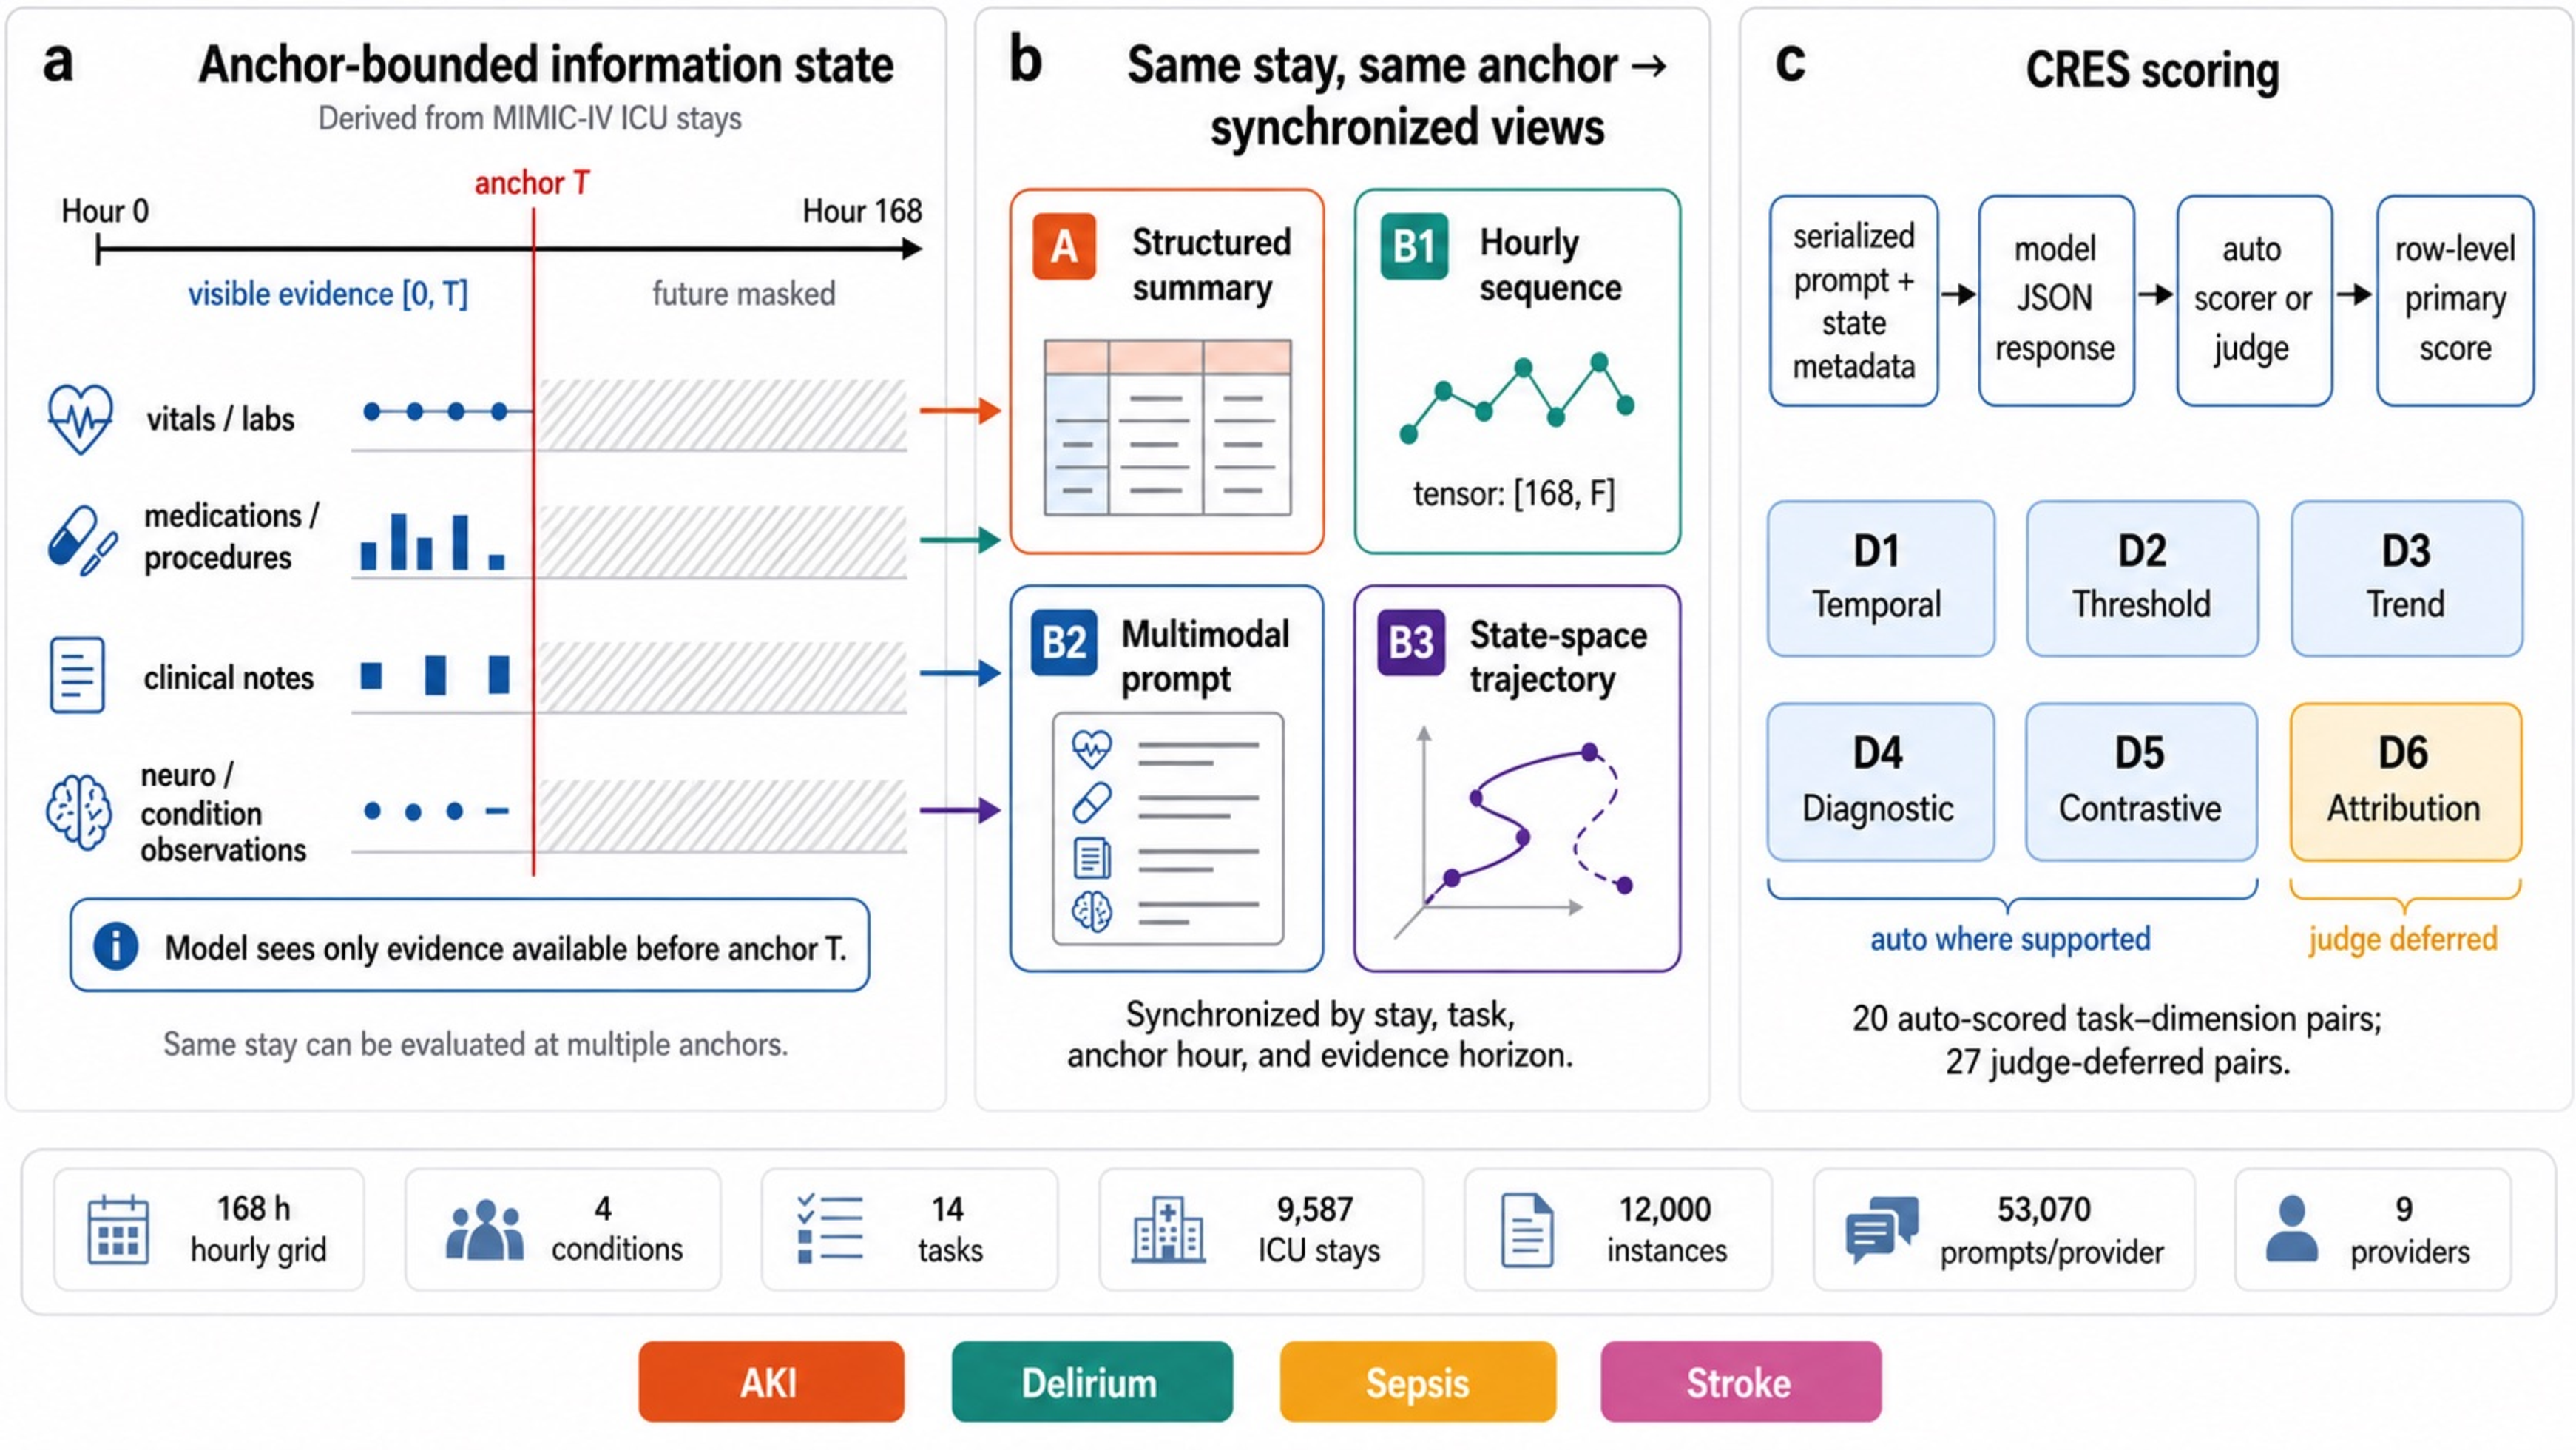
\includegraphics[width=\textwidth]{figures/main/figure1_information_state_anatomy.pdf}
\caption{TIMELY Bench evaluates temporal clinical reasoning by fixing the patient information state at an anchor hour and synchronizing multiple representations of the same ICU stay. Panel a shows that models can only use evidence visible in [0, T], with future information masked. Panel b shows the four synchronized benchmark views: Branch A structured summary, Branch B1 hourly sequence, Branch B2 multimodal EHR prompt, and Branch B3 state-space trajectory. Panel c shows how a Clinical Reasoning Evaluation Suite (CRES) instance maps a stay, task, dimension, and anchor into a serialized prompt, JSON response, and scorer. The bottom scale strip summarizes the frozen evaluation scale.}
\label{fig:architecture}
\end{figure*}

\FloatBarrier

\section{Results}

Results are organized around the three research questions: representation structure, condition-specific difficulty, and model-family differences. We then report CRES dimension behavior, confidence behavior, trajectory-template strata, and judge-rated response quality. This order separates primary benchmark findings from secondary diagnostic analyses.

\subsection{Dataset scale and benchmark composition}

TIMELY Bench is a multi-condition benchmark rather than a repeated binary prediction template. The full release covered 2,456,896 AKI task instances from 49,920 ICU stays, 1,512,502 delirium instances from 21,628 stays, 898,560 sepsis instances from 29,713 stays, and 61,111 stroke instances from 5,318 stays (Table~\ref{tab:dataset_condition}). AKI, delirium, and sepsis each contributed two onset- or state-oriented tasks on a common temporal scaffold; stroke contributed eight tasks split between Layer 1 temporal prediction and Layer 2 retrospective or extraction tasks (Table~\ref{tab:dataset_task}).

Representation availability differed by condition family. Branches A, B1, and B2 were available for all four conditions, whereas B3 and the physiology-template layer were available only for AKI, delirium, and sepsis. Stroke retained anchor-bounded multimodal prompts but was not forced into a phase-template stack because its progression signals were organized around neurological deficit structure, laterality, imaging concordance, and retrospective discharge synthesis.

Task balance also varied. Positive rates ranged from 0.98\% for AKI-S1 and 1.66\% for SEP-T1 to approximately 21--22\% for the delirium tasks; stroke combined binary, categorical, and numeric extraction settings. The frozen formal sample contained 12,000 benchmark instances from 9,587 ICU stays, capped at two anchors per stay per task where applicable. Expanding these instances across the supported task-dimension map yielded 53,070 \texttt{full\_multimodal} prompts per provider.

Prompt length was clinically variable but feasible for the frozen provider set. The median \texttt{full\_multimodal} prompt contained approximately 1,724 tokens (interquartile range 807--2,564; range 183--15,040), with a mean of 1,978 tokens. Stroke prompts were longest on average (median 2,359 tokens) and sepsis shortest (1,120). Clinical notes contributed 58.7\% of prompt tokens on average, followed by structured timeline and medication sections.

\begin{table*}[t]
\caption{Dataset statistics. Panel A summarizes condition-level cohort size, task count, task roster, and representation availability.}
\label{tab:dataset_condition}
\centering
\scriptsize
\begin{tabularx}{\textwidth}{@{}lrr>{\raggedright\arraybackslash}X>{\raggedright\arraybackslash}Xc@{}}
\toprule
Condition & Instances & Unique stays & Tasks & Representations & B3 \\
\midrule
AKI & 2,456,896 & 49,920 & AKI-S1, AKI-T1 & A/B1/B2/B3 & yes \\
Delirium & 1,512,502 & 21,628 & DEL-S1, DEL-T1 & A/B1/B2/B3 & yes \\
Sepsis & 898,560 & 29,713 & SEP-S1, SEP-T1 & A/B1/B2/B3 & yes \\
Stroke & 61,111 & 5,318 & S-R1, S-R2, S-R3, S-R4, S-T1, S-T2, S-T3, S-T4 & A/B1/B2 & no \\
\botrule
\end{tabularx}
\normalsize
\end{table*}


\addtocounter{table}{-1}
\begingroup
\renewcommand{\theHtable}{table.panelb}
\scriptsize
\begin{longtable}{@{}ll>{\raggedright\arraybackslash}p{2.8cm}rr>{\raggedright\arraybackslash}p{1.8cm}>{\raggedright\arraybackslash}p{3.2cm}@{}}
\caption{Dataset statistics. Panel B summarizes task-level instance counts, unique stays, label summary, and representation availability. Disease prefixes denote AKI, delirium (DEL), sepsis (SEP), and stroke (S); task-family letters after the hyphen denote temporal or prospective tasks (T), secondary state or trajectory tasks (S), and retrospective stroke extraction or synthesis tasks (R).}\label{tab:dataset_task}\\
\toprule
Task & Condition & Layer / mode & Instances & Unique stays & Label summary & Representations \\
\midrule
\endfirsthead
\toprule
Task & Condition & Layer / mode & Instances & Unique stays & Label summary & Representations \\
\midrule
\endhead
AKI-S1 & AKI & single-layer temporal & 1,764,883 & 48,461 & 0.98\% & A/B1/B2/B3 \\
AKI-T1 & AKI & single-layer temporal & 692,013 & 40,915 & 8.46\% & A/B1/B2/B3 \\
DEL-S1 & Delirium & single-layer temporal & 756,251 & 21,628 & 22.03\% & A/B1/B2/B3 \\
DEL-T1 & Delirium & single-layer temporal & 756,251 & 21,628 & 21.10\% & A/B1/B2/B3 \\
SEP-S1 & Sepsis & single-layer temporal & 27,003 & 11,715 & 21.11\% & A/B1/B2/B3 \\
SEP-T1 & Sepsis & single-layer temporal & 871,557 & 26,517 & 1.66\% & A/B1/B2/B3 \\
S-R1 & Stroke & Layer 2 retrospective & 3,912 & 3,912 & 5 classes & B2 \\
S-R2 & Stroke & Layer 2 retrospective & 3,912 & 3,912 & 4 classes & B2 \\
S-R3 & Stroke & Layer 2 retrospective & 277 & 277 & median=2.5 & B2 \\
S-R4 & Stroke & Layer 2 retrospective & 3,912 & 3,912 & 8.79\% & B2 \\
S-T1 & Stroke & Layer 1 temporal & 36,519 & 4,792 & 14.25\% & A/B1/B2 \\
S-T2 & Stroke & Layer 1 temporal & 4,952 & 4,952 & 5 classes & A/B1/B2 \\
S-T3 & Stroke & Layer 1 temporal & 2,651 & 2,651 & 3 classes & A/B1/B2 \\
S-T4 & Stroke & Layer 1 temporal & 4,976 & 4,976 & 16 classes & A/B1/B2 \\
\botrule
\end{longtable}
\normalsize

\endgroup

\FloatBarrier

\subsection{Explicit temporal structure helped selectively}

The branch comparison tested RQ1 by asking whether an hourly structured sequence improved over a compact anchor-state summary in conventional baselines. Branch A XGBoost was strong for AKI-S1 (AUROC 0.977), AKI-T1 (0.941), both delirium tasks (0.918 and 0.916), and SEP-T1 (0.950), but weaker for SEP-S1 (0.751) and S-T1 (0.726) (Table~\ref{tab:structured_baselines}).

Explicit hourly sequence modeling did not uniformly dominate. Using the AUROC-selected B1 model for each task as the shared comparator, B1 improved AUROC on only three of seven eligible tasks: AKI-S1, AKI-T1, and SEP-T1. It improved AUPRC on only one task, AKI-T1, where BiLSTM-attention increased AUROC from 0.941 to 0.949 and AUPRC from 0.595 to 0.603. The largest B1 deficit was SEP-S1, where B1 underperformed A by 0.047 AUROC and 0.057 AUPRC. Temporal structure helped selectively, not automatically.

This result is important because the branch comparison is not an LLM prompt ablation. It isolates the structured-data question of whether preserving the hourly sequence improves over summarizing the anchor state. The answer was task-dependent: sequence models helped when evolving physiology was recoverable from the hourly grid, but not when the summary already captured the signal or when the sequence introduced sparse, noisy observations.

\begin{table*}[t]
\caption{Structured baselines on eligible binary tasks. Five-fold subject-level cross-validation results for Branch A and Branch B1, reported as mean AUROC and AUPRC.}
\label{tab:structured_baselines}
\centering
\scriptsize
\begin{tabular}{@{}llllrr@{}}
\toprule
Task & Condition & Branch & Model & AUROC & AUPRC \\
\midrule
AKI-S1 & AKI & A & xgboost & 0.977 & 0.372 \\
AKI-S1 & AKI & B1 & temporal\_transformer & 0.978 & 0.346 \\
AKI-S1 & AKI & B1 & bilstm\_attention & 0.977 & 0.339 \\
AKI-T1 & AKI & A & xgboost & 0.941 & 0.595 \\
AKI-T1 & AKI & B1 & bilstm\_attention & 0.949 & 0.603 \\
AKI-T1 & AKI & B1 & temporal\_transformer & 0.941 & 0.562 \\
DEL-S1 & Delirium & A & xgboost & 0.918 & 0.702 \\
DEL-S1 & Delirium & B1 & temporal\_transformer & 0.911 & 0.689 \\
DEL-S1 & Delirium & B1 & bilstm\_attention & 0.910 & 0.702 \\
DEL-T1 & Delirium & A & xgboost & 0.916 & 0.692 \\
DEL-T1 & Delirium & B1 & bilstm\_attention & 0.908 & 0.659 \\
DEL-T1 & Delirium & B1 & temporal\_transformer & 0.894 & 0.615 \\
SEP-S1 & Sepsis & A & xgboost & 0.751 & 0.465 \\
SEP-S1 & Sepsis & B1 & bilstm\_attention & 0.704 & 0.408 \\
SEP-S1 & Sepsis & B1 & temporal\_transformer & 0.643 & 0.338 \\
SEP-T1 & Sepsis & A & xgboost & 0.950 & 0.329 \\
SEP-T1 & Sepsis & B1 & bilstm\_attention & 0.953 & 0.275 \\
SEP-T1 & Sepsis & B1 & temporal\_transformer & 0.948 & 0.258 \\
S-T1 & Stroke & A & xgboost & 0.726 & 0.251 \\
S-T1 & Stroke & B1 & bilstm\_attention & 0.707 & 0.247 \\
S-T1 & Stroke & B1 & temporal\_transformer & 0.676 & 0.230 \\
\botrule
\end{tabular}
\normalsize
\end{table*}


\begin{figure*}[t]
\centering
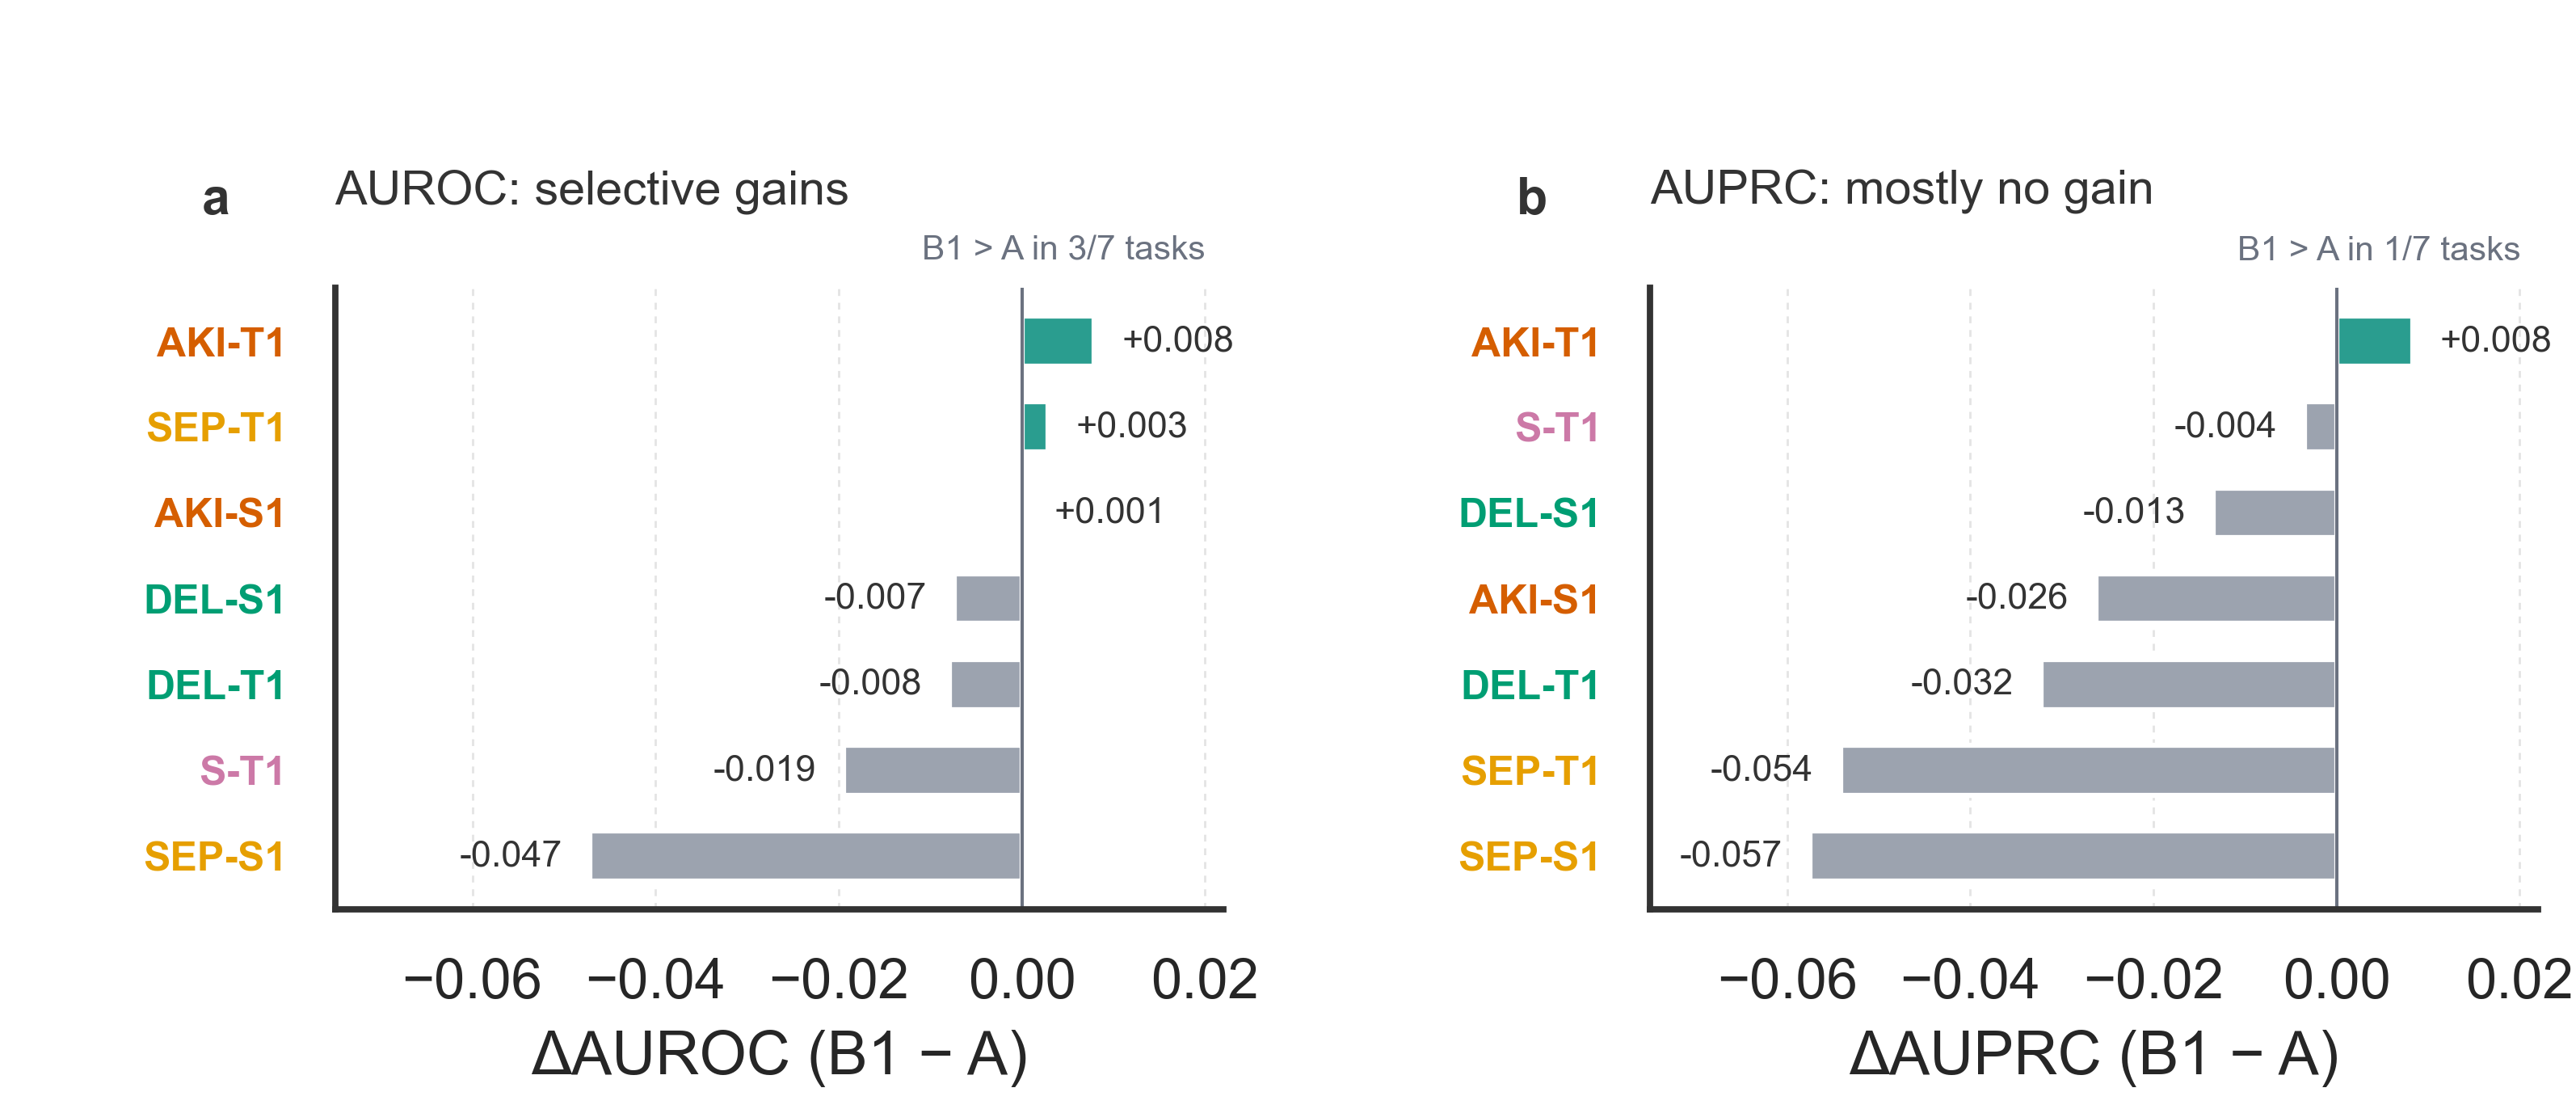
\includegraphics[width=\textwidth]{figures/main/figure2_branch_delta_first.png}
\caption{Explicit hourly sequence modeling improved performance only selectively, indicating that the value of temporal detail was task-dependent. Panel a shows delta AUROC and panel b shows delta AUPRC, both computed as Branch B1 minus Branch A for the seven eligible binary tasks. For each task, Branch B1 is represented by the B1 model selected by AUROC, and both AUROC and AUPRC deltas are computed using that same selected B1 comparator relative to Branch A. B1 improved AUROC in 3/7 tasks (AKI-S1, AKI-T1, SEP-T1) and improved AUPRC in 1/7 tasks (AKI-T1 only). Negative deltas indicate tasks where the simpler structured baseline outperformed the explicit hourly-sequence model.}
\label{fig:branch_comparison}
\end{figure*}

\FloatBarrier

\subsection{General-purpose models led the aggregate ranking}

The provider comparison tested RQ3 by evaluating whether medical-domain adaptation improved anchor-bounded temporal reasoning. The formal set included nine frozen providers: two Tier 1A closed general-purpose API models, three Tier 1B general-purpose open or semi-open models, and four Tier 2 medical-domain adapted models. Tier labels were analysis strata rather than performance-derived categories. Macro primary score was the equal-weight mean over 20 supported task-dimension scores, not a row-weighted average.

Overall macro primary score ranged from 0.489 to 0.655 (Table~\ref{tab:provider_ranking}). Gemini 3.1 Pro led at 0.655, followed by Gemma4-26B (0.646), DeepSeek Chat (0.635), Qwen3.5 (0.634), and GPT-5.4 (0.626). The best Tier 2 model, MedGemma-4B, reached 0.535, below all Tier 1A and Tier 1B providers. Aloe-70B, Meditron3-8B, and Aloe-7B followed at 0.519, 0.510, and 0.489.

Condition-level summaries explain why overall averages should be read cautiously (Table~\ref{tab:condition_summary}; Fig.~\ref{fig:provider_comparison}). Delirium was near ceiling for several providers, AKI favored GPT-5.4 and Gemini 3.1 Pro, sepsis favored several Tier 1B providers, and stroke remained difficult for all tiers. Temporal clinical reasoning therefore did not behave as one uniform capability.

The condition pattern also prevents an over-simple interpretation of the tier gap. Tier 2 models did not fail uniformly on every slice, and some condition-level comparisons were close. The robust statement is that the tested medical-domain adapted models did not outperform the general-purpose groups in aggregate or at the leading-provider level under this frozen evaluation design.

\begin{table*}[t]
\caption{Frozen cross-provider comparative ranking across the nine-provider formal comparative set. Pair wins denote the number of supported task-dimension pairs for which the provider achieved the highest primary score within its tier; ties are counted for all co-winning providers.}
\label{tab:provider_ranking}
\centering
\scriptsize
\begin{tabular}{@{}llrrrr@{}}
\toprule
Provider & Tier & Macro score & Pair wins & Avg latency (s) & Total tokens \\
\midrule
Gemini 3.1 Pro & Tier 1A & 0.655 & 16 & 15.938 & 343,643,633 \\
Gemma4-26B & Tier 1B & 0.646 & 12 & 30.038 & 277,833,535 \\
DeepSeek Chat & Tier 1B & 0.635 & 10 & 12.711 & 261,196,668 \\
Qwen3.5 & Tier 1B & 0.634 & 4 & 4.843 & 285,969,716 \\
GPT-5.4 & Tier 1A & 0.626 & 9 & 11.401 & 264,064,840 \\
MedGemma-4B & Tier 2 & 0.535 & 8 & 71.572 & 285,394,344 \\
Aloe-70B & Tier 2 & 0.519 & 11 & 5.710 & 258,039,766 \\
Meditron3-8B & Tier 2 & 0.510 & 7 & 3.198 & 259,948,539 \\
Aloe-7B & Tier 2 & 0.489 & 7 & 2.759 & 282,111,131 \\
\botrule
\end{tabular}
\normalsize
\end{table*}


\FloatBarrier

\scriptsize
\begin{longtable}{@{}llllr@{}}
\caption{Condition-level comparative summary. Condition-stratified provider performance summarized as macro primary score within each condition family.}\label{tab:condition_summary}\\
\toprule
Provider & Tier & Condition & Macro score & Pairs \\
\midrule
\endfirsthead
\toprule
Provider & Tier & Condition & Macro score & Pairs \\
\midrule
\endhead
GPT-5.4 & Tier 1A & AKI & 0.789 & 5 \\
Gemini 3.1 Pro & Tier 1A & AKI & 0.786 & 5 \\
DeepSeek Chat & Tier 1B & AKI & 0.753 & 5 \\
Gemma4-26B & Tier 1B & AKI & 0.708 & 5 \\
Qwen3.5 & Tier 1B & AKI & 0.679 & 5 \\
MedGemma-4B & Tier 2 & AKI & 0.477 & 5 \\
Aloe-70B & Tier 2 & AKI & 0.458 & 5 \\
Meditron3-8B & Tier 2 & AKI & 0.418 & 5 \\
Aloe-7B & Tier 2 & AKI & 0.342 & 5 \\
DeepSeek Chat & Tier 1B & Delirium & 1.000 & 3 \\
Gemini 3.1 Pro & Tier 1A & Delirium & 1.000 & 3 \\
GPT-5.4 & Tier 1A & Delirium & 1.000 & 3 \\
Aloe-70B & Tier 2 & Delirium & 1.000 & 3 \\
Gemma4-26B & Tier 1B & Delirium & 0.996 & 3 \\
Qwen3.5 & Tier 1B & Delirium & 0.993 & 3 \\
Aloe-7B & Tier 2 & Delirium & 0.964 & 3 \\
Meditron3-8B & Tier 2 & Delirium & 0.958 & 3 \\
MedGemma-4B & Tier 2 & Delirium & 0.883 & 3 \\
Gemma4-26B & Tier 1B & Sepsis & 0.833 & 4 \\
Qwen3.5 & Tier 1B & Sepsis & 0.822 & 4 \\
Gemini 3.1 Pro & Tier 1A & Sepsis & 0.802 & 4 \\
DeepSeek Chat & Tier 1B & Sepsis & 0.795 & 4 \\
GPT-5.4 & Tier 1A & Sepsis & 0.750 & 4 \\
MedGemma-4B & Tier 2 & Sepsis & 0.714 & 4 \\
Meditron3-8B & Tier 2 & Sepsis & 0.686 & 4 \\
Aloe-7B & Tier 2 & Sepsis & 0.632 & 4 \\
Aloe-70B & Tier 2 & Sepsis & 0.556 & 4 \\
Gemma4-26B & Tier 1B & Stroke & 0.382 & 8 \\
Qwen3.5 & Tier 1B & Stroke & 0.376 & 8 \\
Gemini 3.1 Pro & Tier 1A & Stroke & 0.371 & 8 \\
Aloe-70B & Tier 2 & Stroke & 0.359 & 8 \\
MedGemma-4B & Tier 2 & Stroke & 0.350 & 8 \\
DeepSeek Chat & Tier 1B & Stroke & 0.344 & 8 \\
Aloe-7B & Tier 2 & Stroke & 0.331 & 8 \\
GPT-5.4 & Tier 1A & Stroke & 0.321 & 8 \\
Meditron3-8B & Tier 2 & Stroke & 0.312 & 8 \\
\botrule
\end{longtable}
\normalsize


\begin{figure*}[t]
\centering
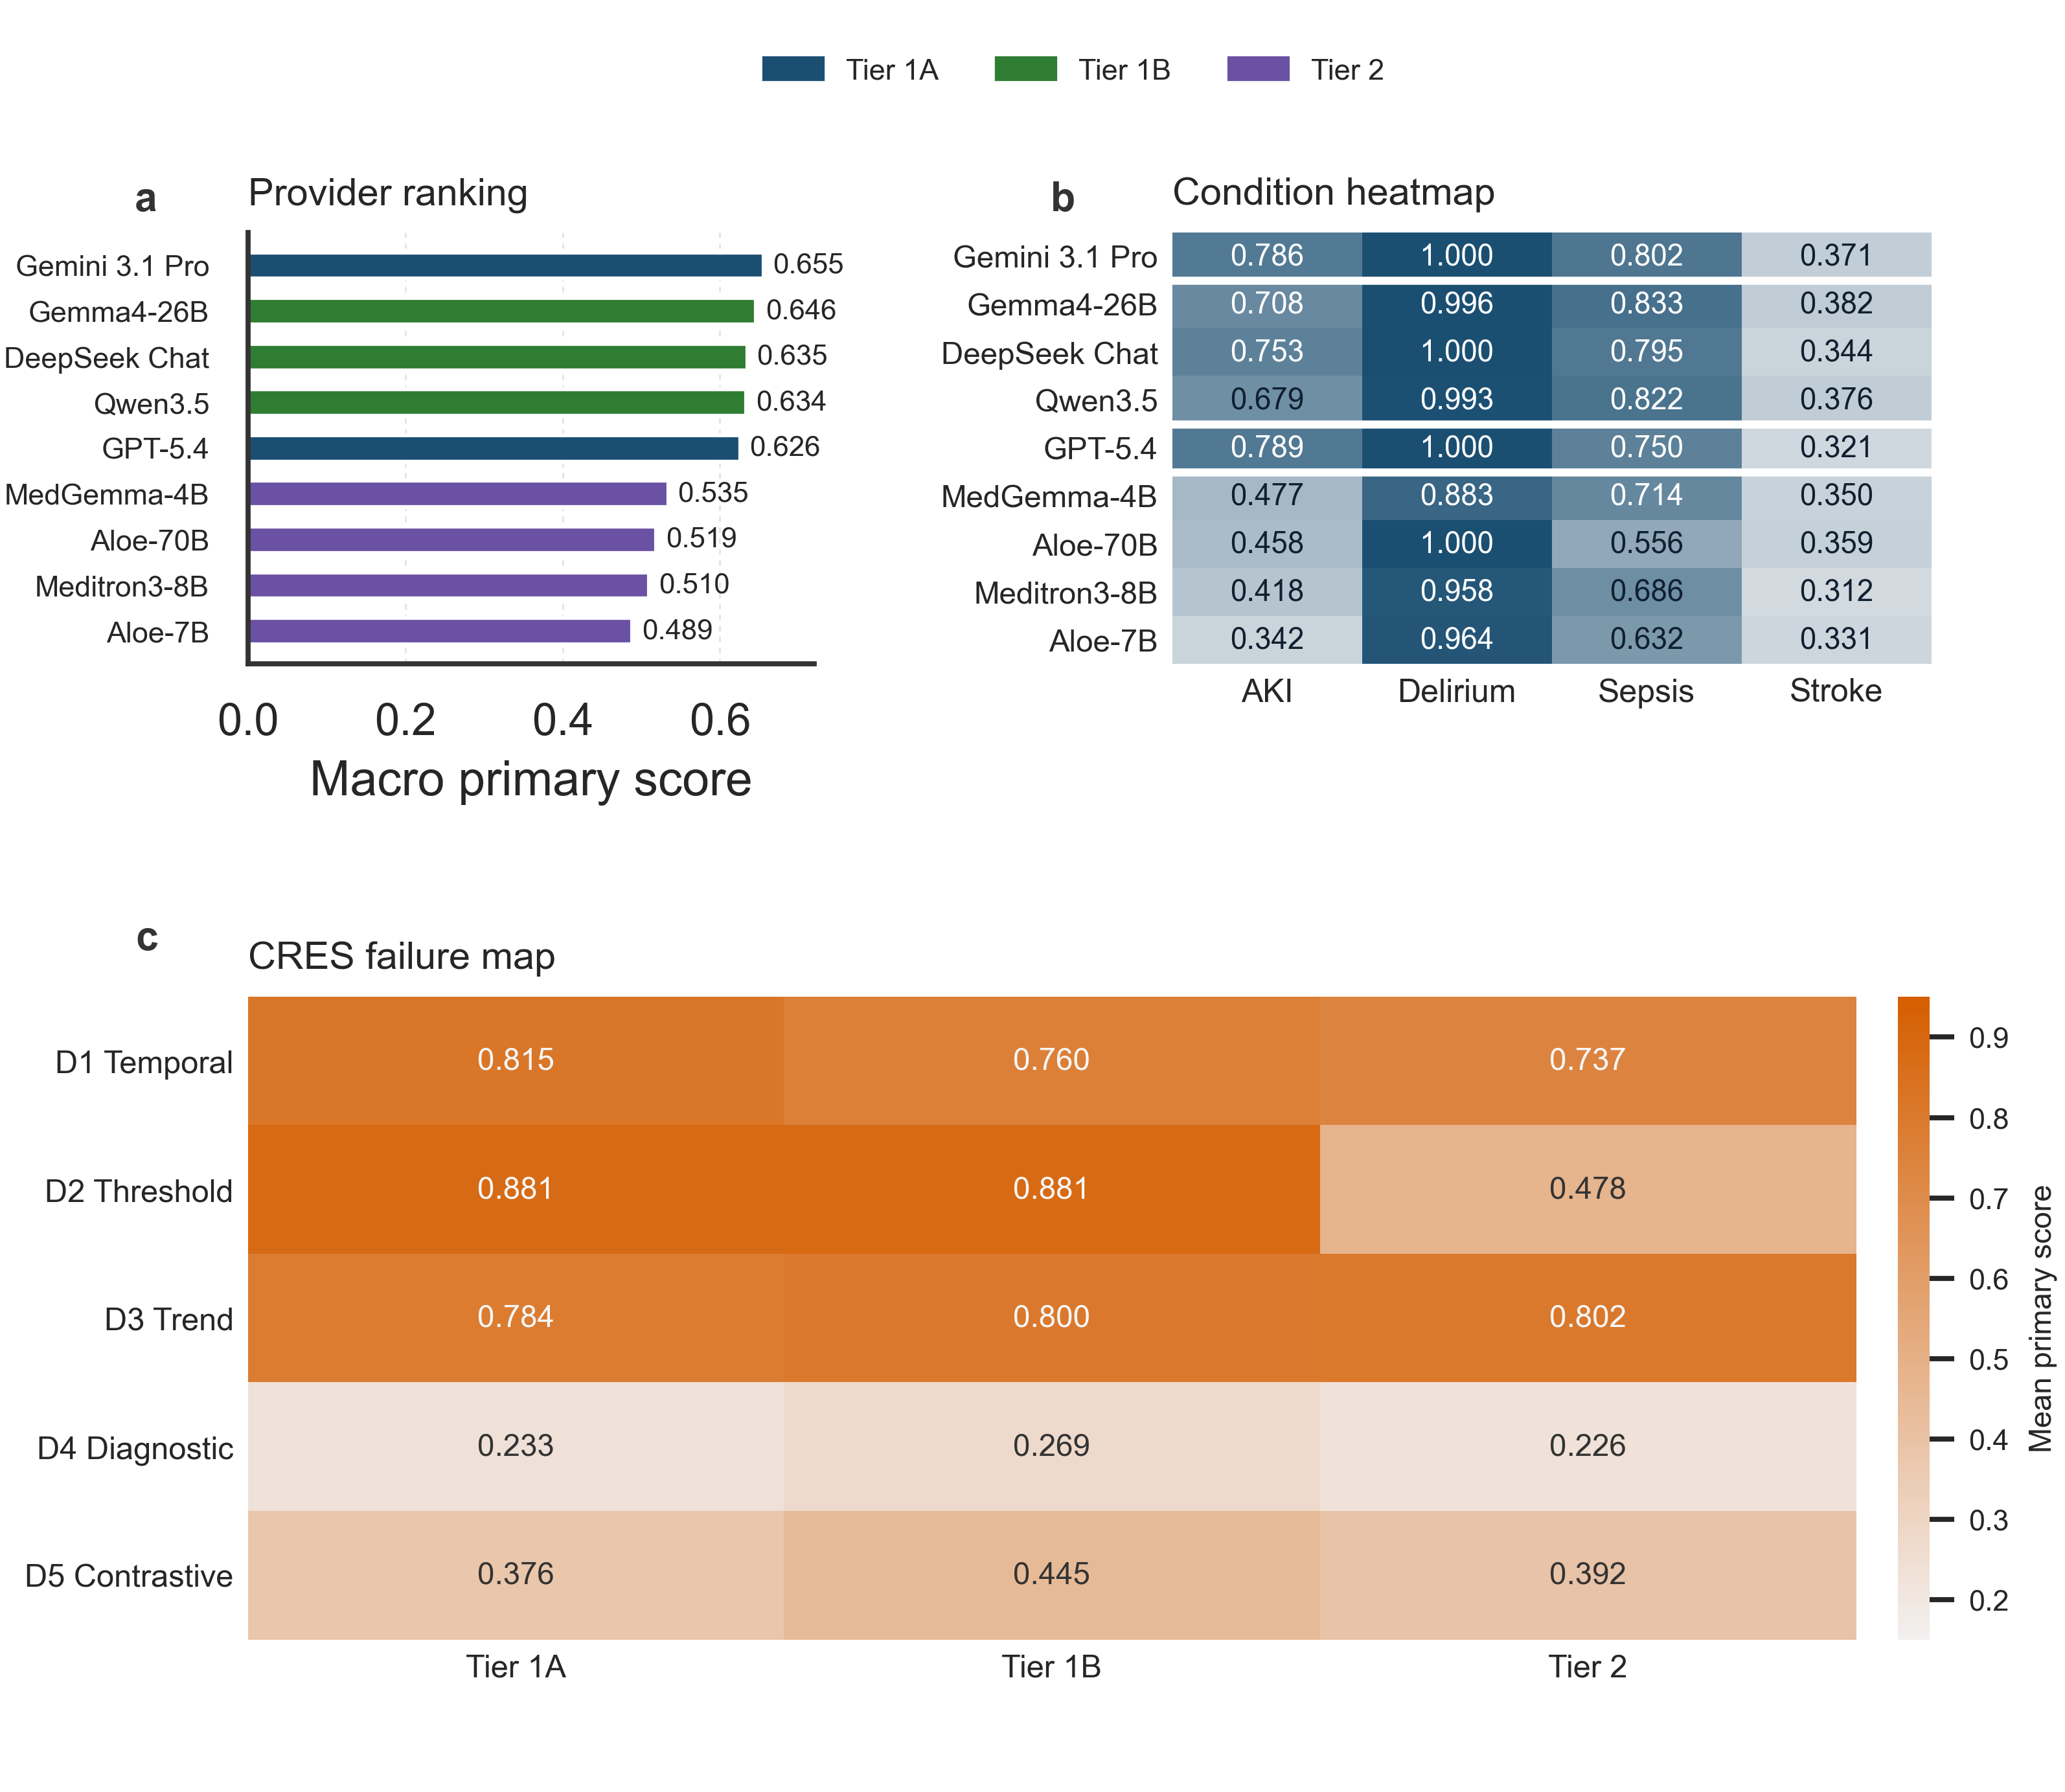
\includegraphics[width=\textwidth]{figures/main/figure3_provider_condition_cres.png}
\caption{General-purpose models led the frozen comparison, while Clinical Reasoning Evaluation Suite (CRES) stratification showed dimension-specific failure patterns. Panel a shows overall macro primary score by provider, with bars colored by model tier. Panel b shows condition-level macro primary scores across AKI, delirium, sepsis, and stroke. Panel c shows mean primary score by CRES dimension and provider tier for auto-scored dimensions D1--D5. D1--D5 are auto-scored where supported; D6 attribution is judge-deferred and excluded from primary auto-scoring.}
\label{fig:provider_comparison}
\end{figure*}

\FloatBarrier

\subsection{Per-dimension CRES analysis exposed distinct reasoning failure modes}

CRES separated aggregate performance into clinically interpretable operations (Table~\ref{tab:cres_dimensions}). Formal auto-scoring covered 20 supported task-dimension pairs across D1--D5; 27 pairs and D6 attribution were deferred to judge evaluation or qualitative inspection.

Across providers, D3 trend reasoning was strongest (mean primary score 0.797), followed by D1 temporal localization (0.762) and D2 threshold reasoning (0.702). D5 contrastive reasoning was lower (0.406), and D4 diagnostic discrimination was weakest (0.242). This ordering is clinically plausible: trend classification can be straightforward once the relevant trajectory is visible, whereas diagnostic discrimination requires choosing among overlapping explanations under partial evidence.

The largest tier separation appeared in D2. Tier 1A and Tier 1B both averaged approximately 0.881 on threshold reasoning, whereas Tier 2 averaged 0.478. The pattern was not uniform weakness: Tier 2 was competitive on D3 trend reasoning (0.802) and comparatively stronger on D5. Condition-level dimension results reinforced this interpretation. D1 was near ceiling for delirium and sepsis, moderate for AKI, and near floor for stroke; D2 was high for delirium, intermediate for stroke and AKI, and lower for sepsis, where the target combines MAP, vasopressor exposure, lactate availability, and onset chronology.

Per-dimension reporting is therefore not a cosmetic decomposition of the leaderboard. It identifies which clinical operation fails. A model that can classify a visible trend may still miss a guideline-like threshold, and a model that localizes an event may still misattribute the clinical mechanism. This is why TIMELY Bench reports CRES dimensions alongside task and condition summaries.

\subsection{Confidence behavior varied independently of raw accuracy}

Confidence behavior separated providers in a way that primary score alone did not. GPT-5.4 marked 37,086 of 53,070 outputs as \texttt{high} confidence (69.9\%), whereas Gemini 3.1 Pro marked 52,635 outputs as \texttt{high} (99.2\%). DeepSeek Chat was closer to GPT-5.4 at 71.6\%; Qwen3.5 and Gemma4-26B were more compressed at 90.7\% and 94.9\%. Gemini 3.1 Pro led the overall score but used the high-confidence label almost uniformly, making uncertainty-aware triage or selective escalation harder to infer from the response schema.

\subsection{Temporal sensitivity varied by condition}

The temporal stress test examined whether condition difficulty changed across early, middle, and later anchor windows.

Temporal degradation analysis used predefined anchor buckets instead of exact single-hour points: T6 for anchor hours 4--8, T24 for hours 18--30, and T48 for hours 46--50. Any provider-task-bucket cell with fewer than 25 instances was marked as insufficient support and excluded from the main plot. Delirium and stroke do not show a T24 marker in the main figure because the middle bucket failed the support threshold, not because the data were missing.

The temporal pattern was not monotonic (Fig.~\ref{fig:temporal_degradation}). Sepsis displayed a T24 peak before declining again at T48. A plausible explanation is signal concentration: the T24 window disproportionately captures high-information segments around sepsis-to-shock evolution, whereas T48 includes more heterogeneous and partially stabilized stays. The result is more specific than ``earlier is harder'' or ``later is easier.'' Anchor sensitivity depends on where clinically informative signal is concentrated along the trajectory.

\begin{figure*}[t]
\centering
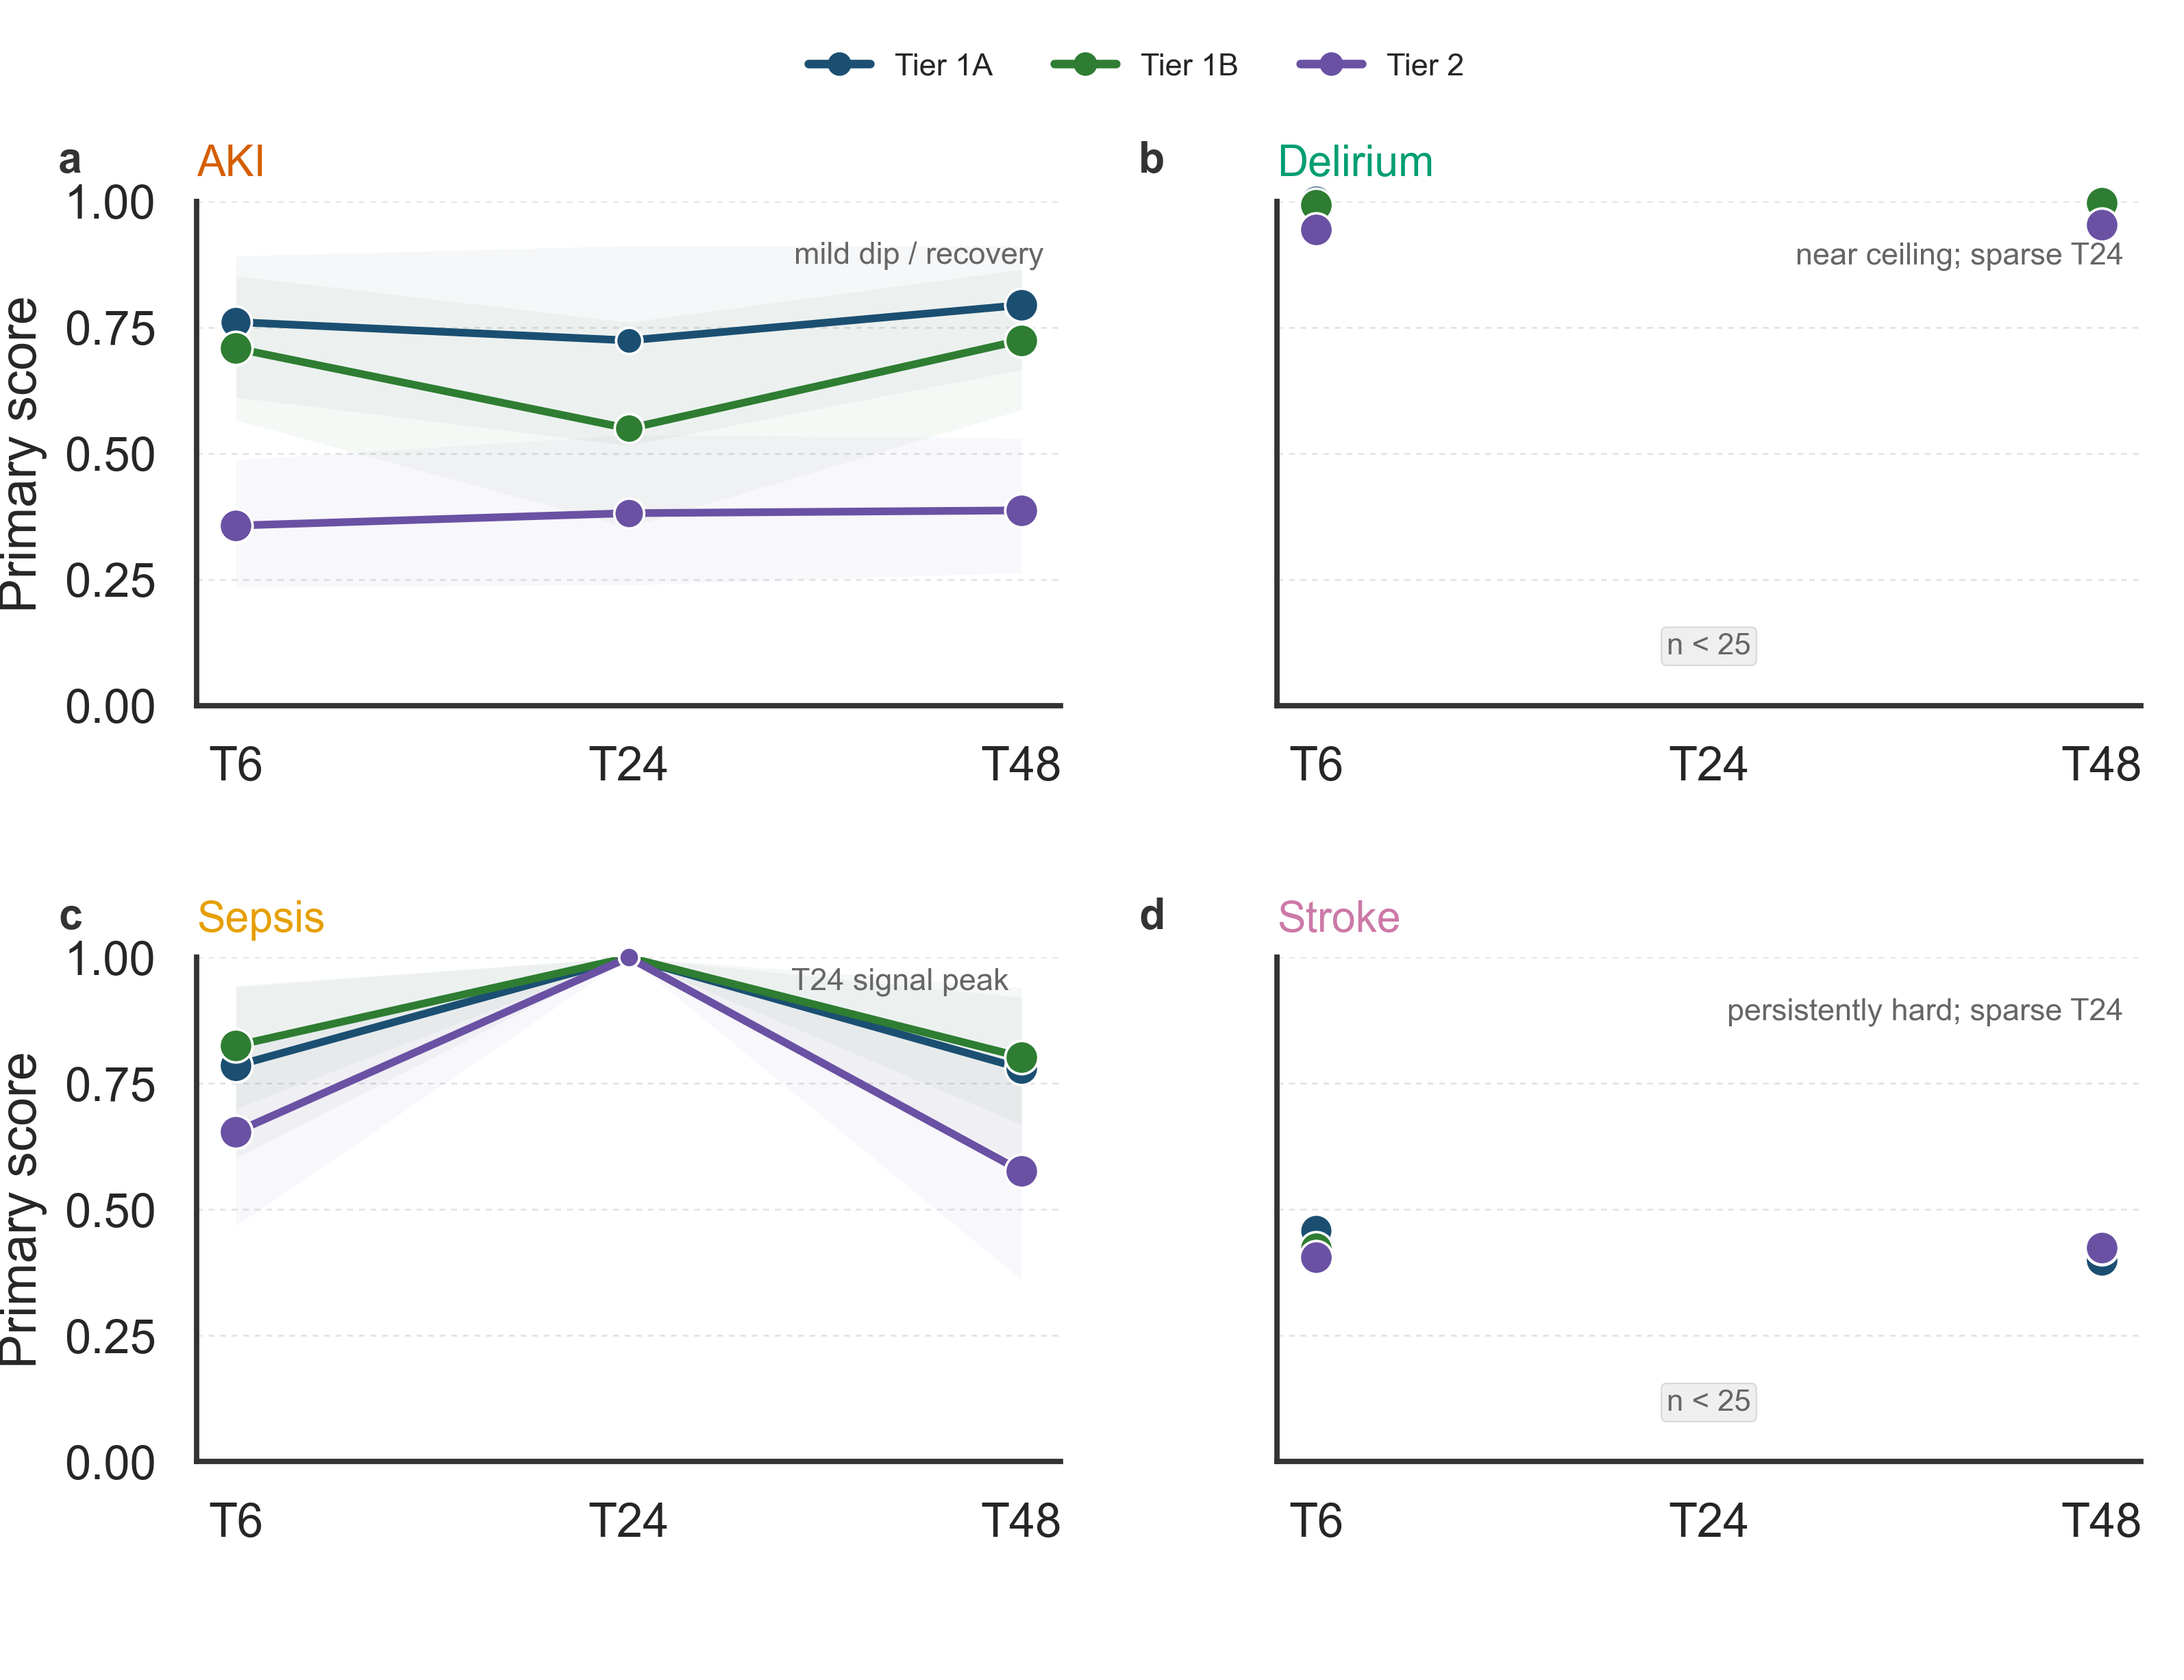
\includegraphics[width=\textwidth]{figures/main/figure4_temporal_stress_test.png}
\caption{Temporal sensitivity varied by condition and was not uniformly monotonic. Mean primary score is shown across predefined temporal buckets T6 (anchor hours 4--8), T24 (18--30), and T48 (46--50), stratified by provider tier and condition. Point size reflects the number of scored instances in each tier-condition-bucket cell, and shaded bands indicate bootstrap uncertainty where available. Cells with fewer than 25 instances were marked as insufficient support rather than treated as missing data. Sepsis showed a T24 signal peak, whereas delirium remained near ceiling and stroke remained persistently difficult.}
\label{fig:temporal_degradation}
\end{figure*}

\FloatBarrier

\subsection{The stroke two-layer split captured a real reasoning boundary}

The stroke analysis separated prospective temporal prediction from retrospective synthesis within the same condition family.

Stroke was designed differently from the other three conditions because it contains two qualitatively distinct reasoning regimes. Layer 1 evaluates anchor-bounded temporal prediction over evolving neurological observations. Layer 2 evaluates retrospective mechanism, strategy, numeric extraction, and complication reasoning using discharge and stay-level context. The empirical results support this split.

Layer 2 outperformed Layer 1 for all nine providers, with a mean Layer 2 minus Layer 1 gain of 0.130 macro primary score (Fig.~\ref{fig:stroke_layers}). The largest gains were observed for MedGemma-4B (+0.240), Gemma4-26B (+0.168), and Aloe-7B (+0.167). Retrospective synthesis from the full documented course was easier than short-horizon temporal stroke prediction under anchor masking. The same clinical story becomes much harder when the model must judge deterioration from partial evolving evidence, which is why stroke was separated into two layers.

\begin{figure*}[t]
\centering
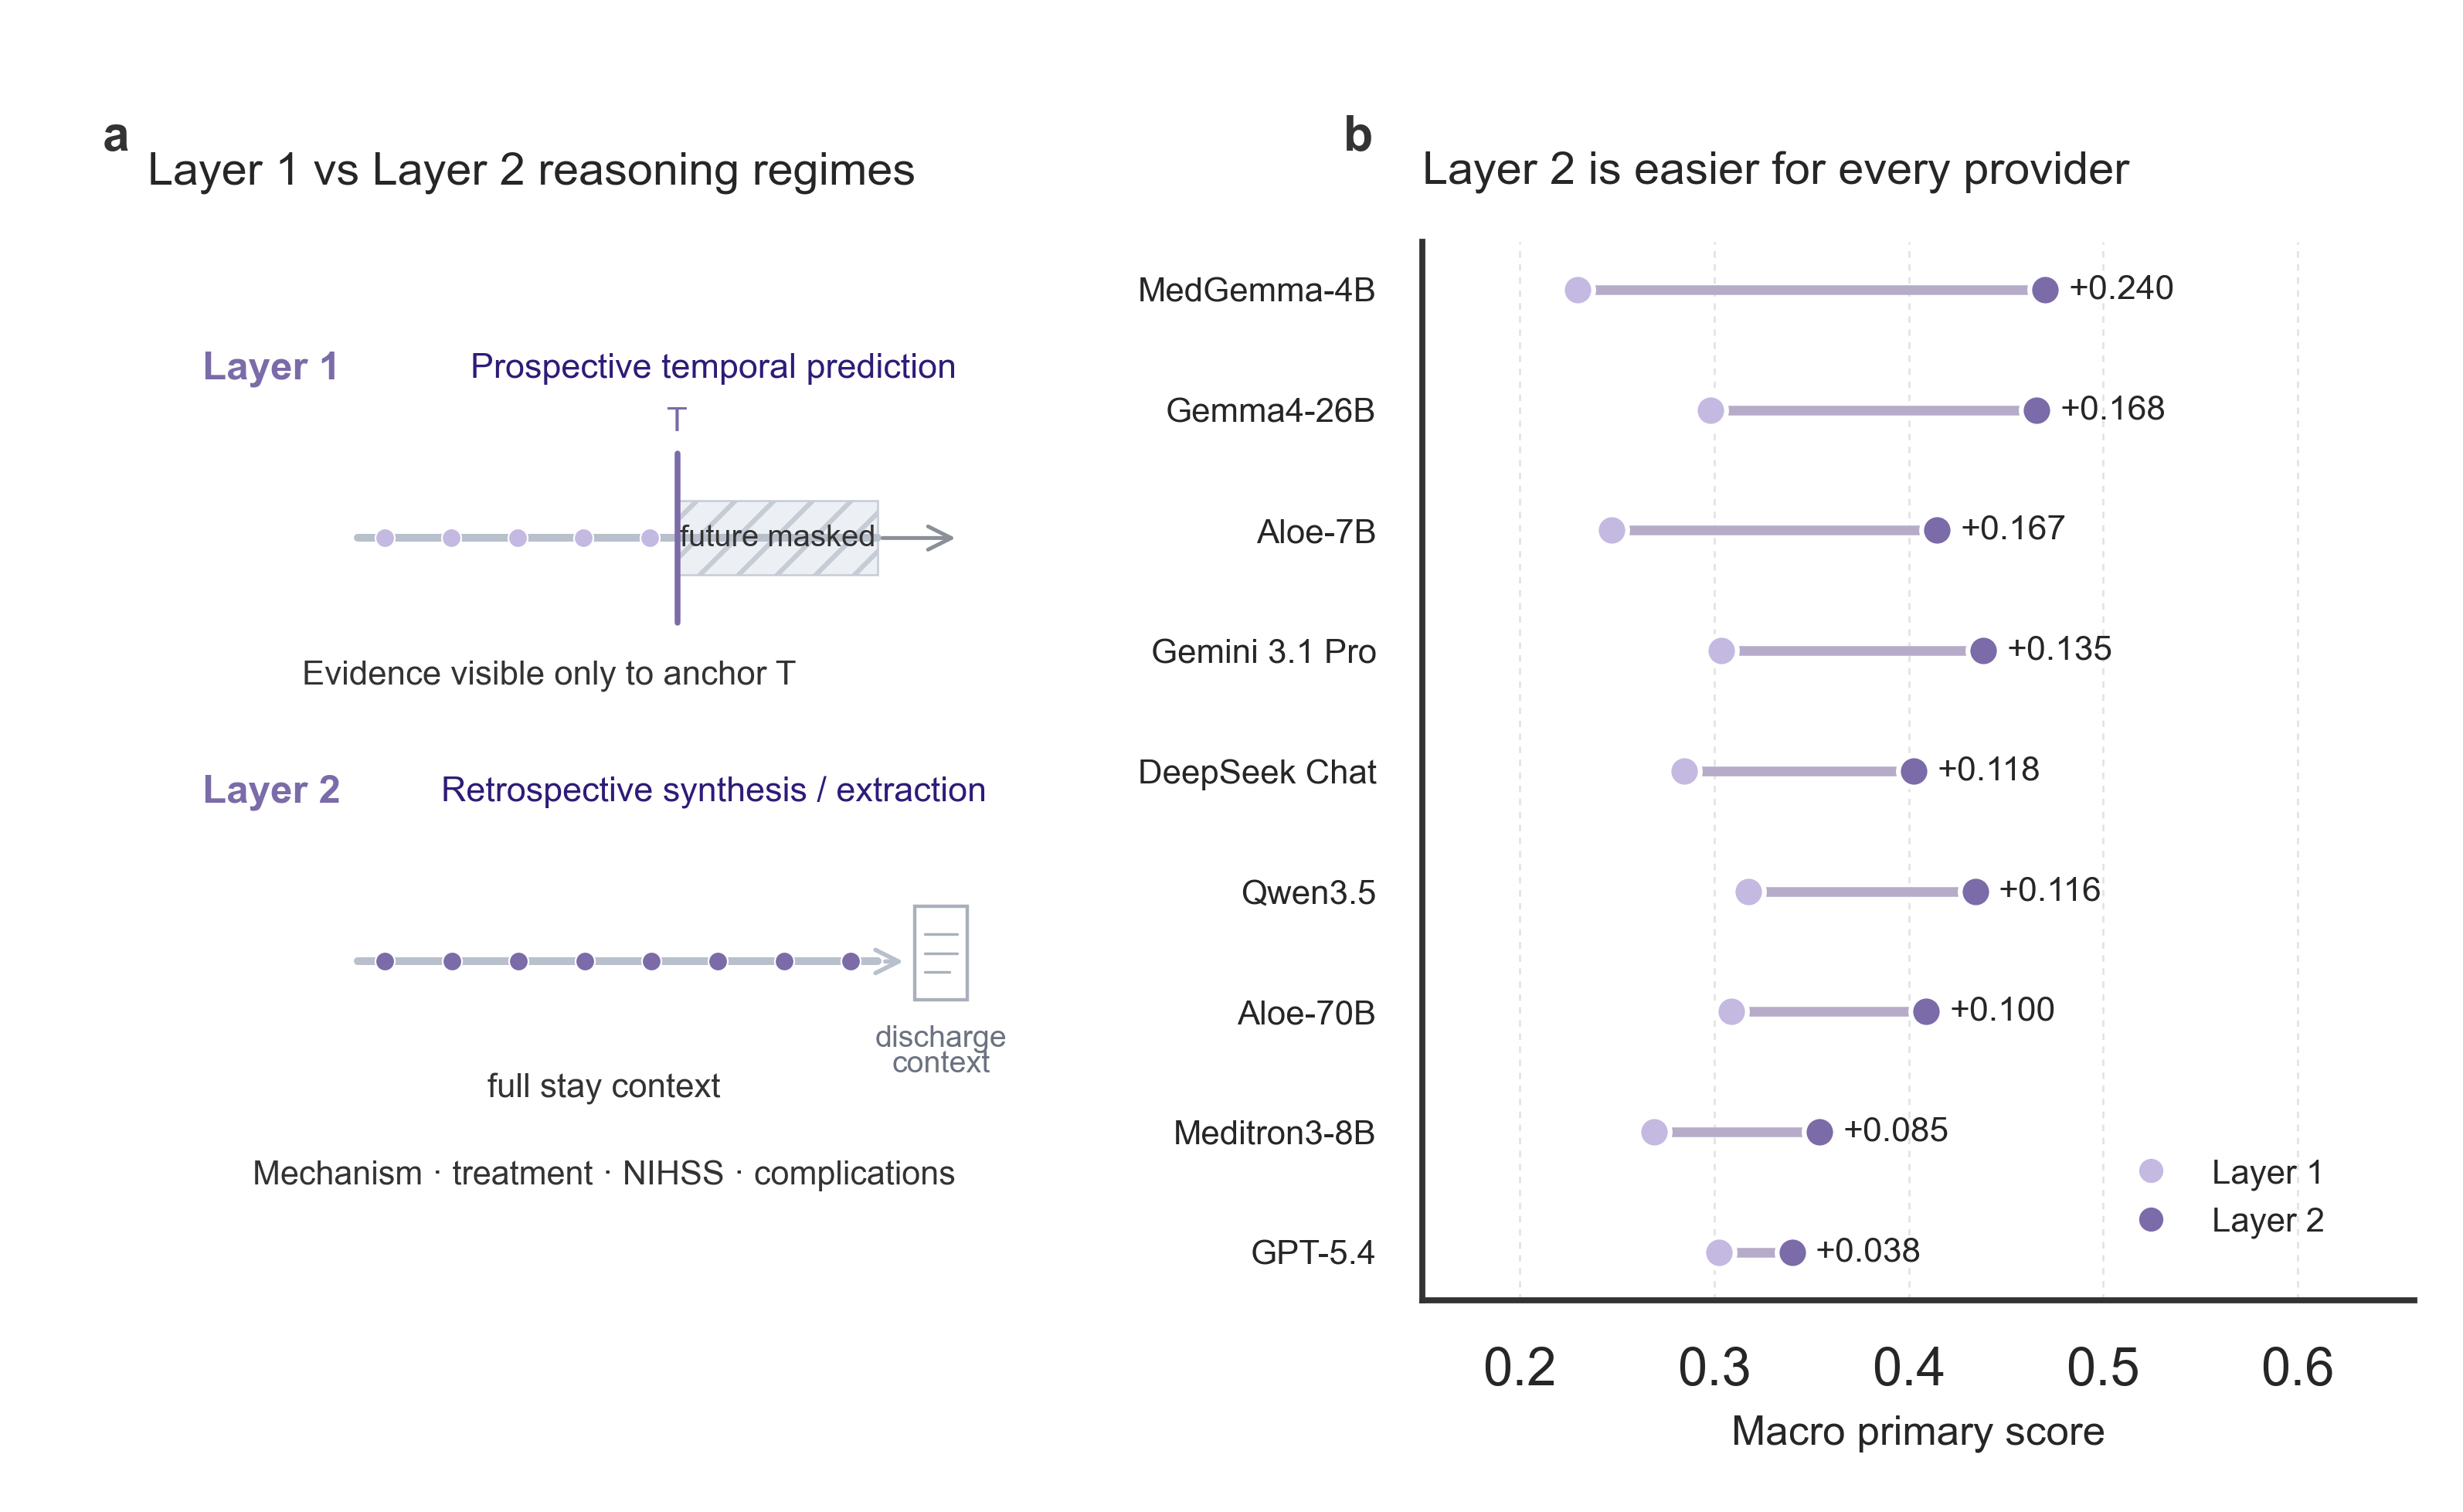
\includegraphics[width=\textwidth]{figures/main/figure5_stroke_layer_mechanism.png}
\caption{The stroke two-layer split captured a real reasoning boundary: retrospective synthesis and extraction were consistently easier than anchor-bounded temporal prediction. Panel a contrasts Layer 1, where only pre-anchor evidence is visible and the future neurological state is masked, with Layer 2, where full stay-level and discharge context support retrospective mechanism, treatment, NIHSS, and complication extraction. Panel b shows provider-level macro primary score for Layer 1 and Layer 2; Layer 2 outperformed Layer 1 for all nine providers. The mean Layer 2 minus Layer 1 gain was approximately +0.130 macro primary score.}
\label{fig:stroke_layers}
\end{figure*}

\FloatBarrier

\subsection{Template support revealed a strong trajectory gradient}

The trajectory-tier analysis tested whether physiology-template support identified clinically meaningful differences in trajectory difficulty.

Trajectory-tier analysis linked model performance to how well a stay matched an executable physiology template. Stay-level template-support coverage was 6\% for AKI, 96\% for delirium, and 37\% for sepsis (Fig.~\ref{fig:trajectory_tier}, panel a). These are not model-performance values; they quantify whether adequate observations were available for template-aligned phase rules.

Row-level performance varied across tiers (Fig.~\ref{fig:trajectory_tier}, panel c). The gradient was strongest for delirium, intermediate for sepsis, and weakest for AKI. AKI also showed a counterintuitive pattern: low-support rows outperformed typical-supported rows, probably because low-support AKI contained more easy non-progression cases while typical-supported rows concentrated clinically dynamic trajectories. The important point is that template support exposes case-mix structure hidden by pooled averages.

\begin{figure*}[t]
\centering
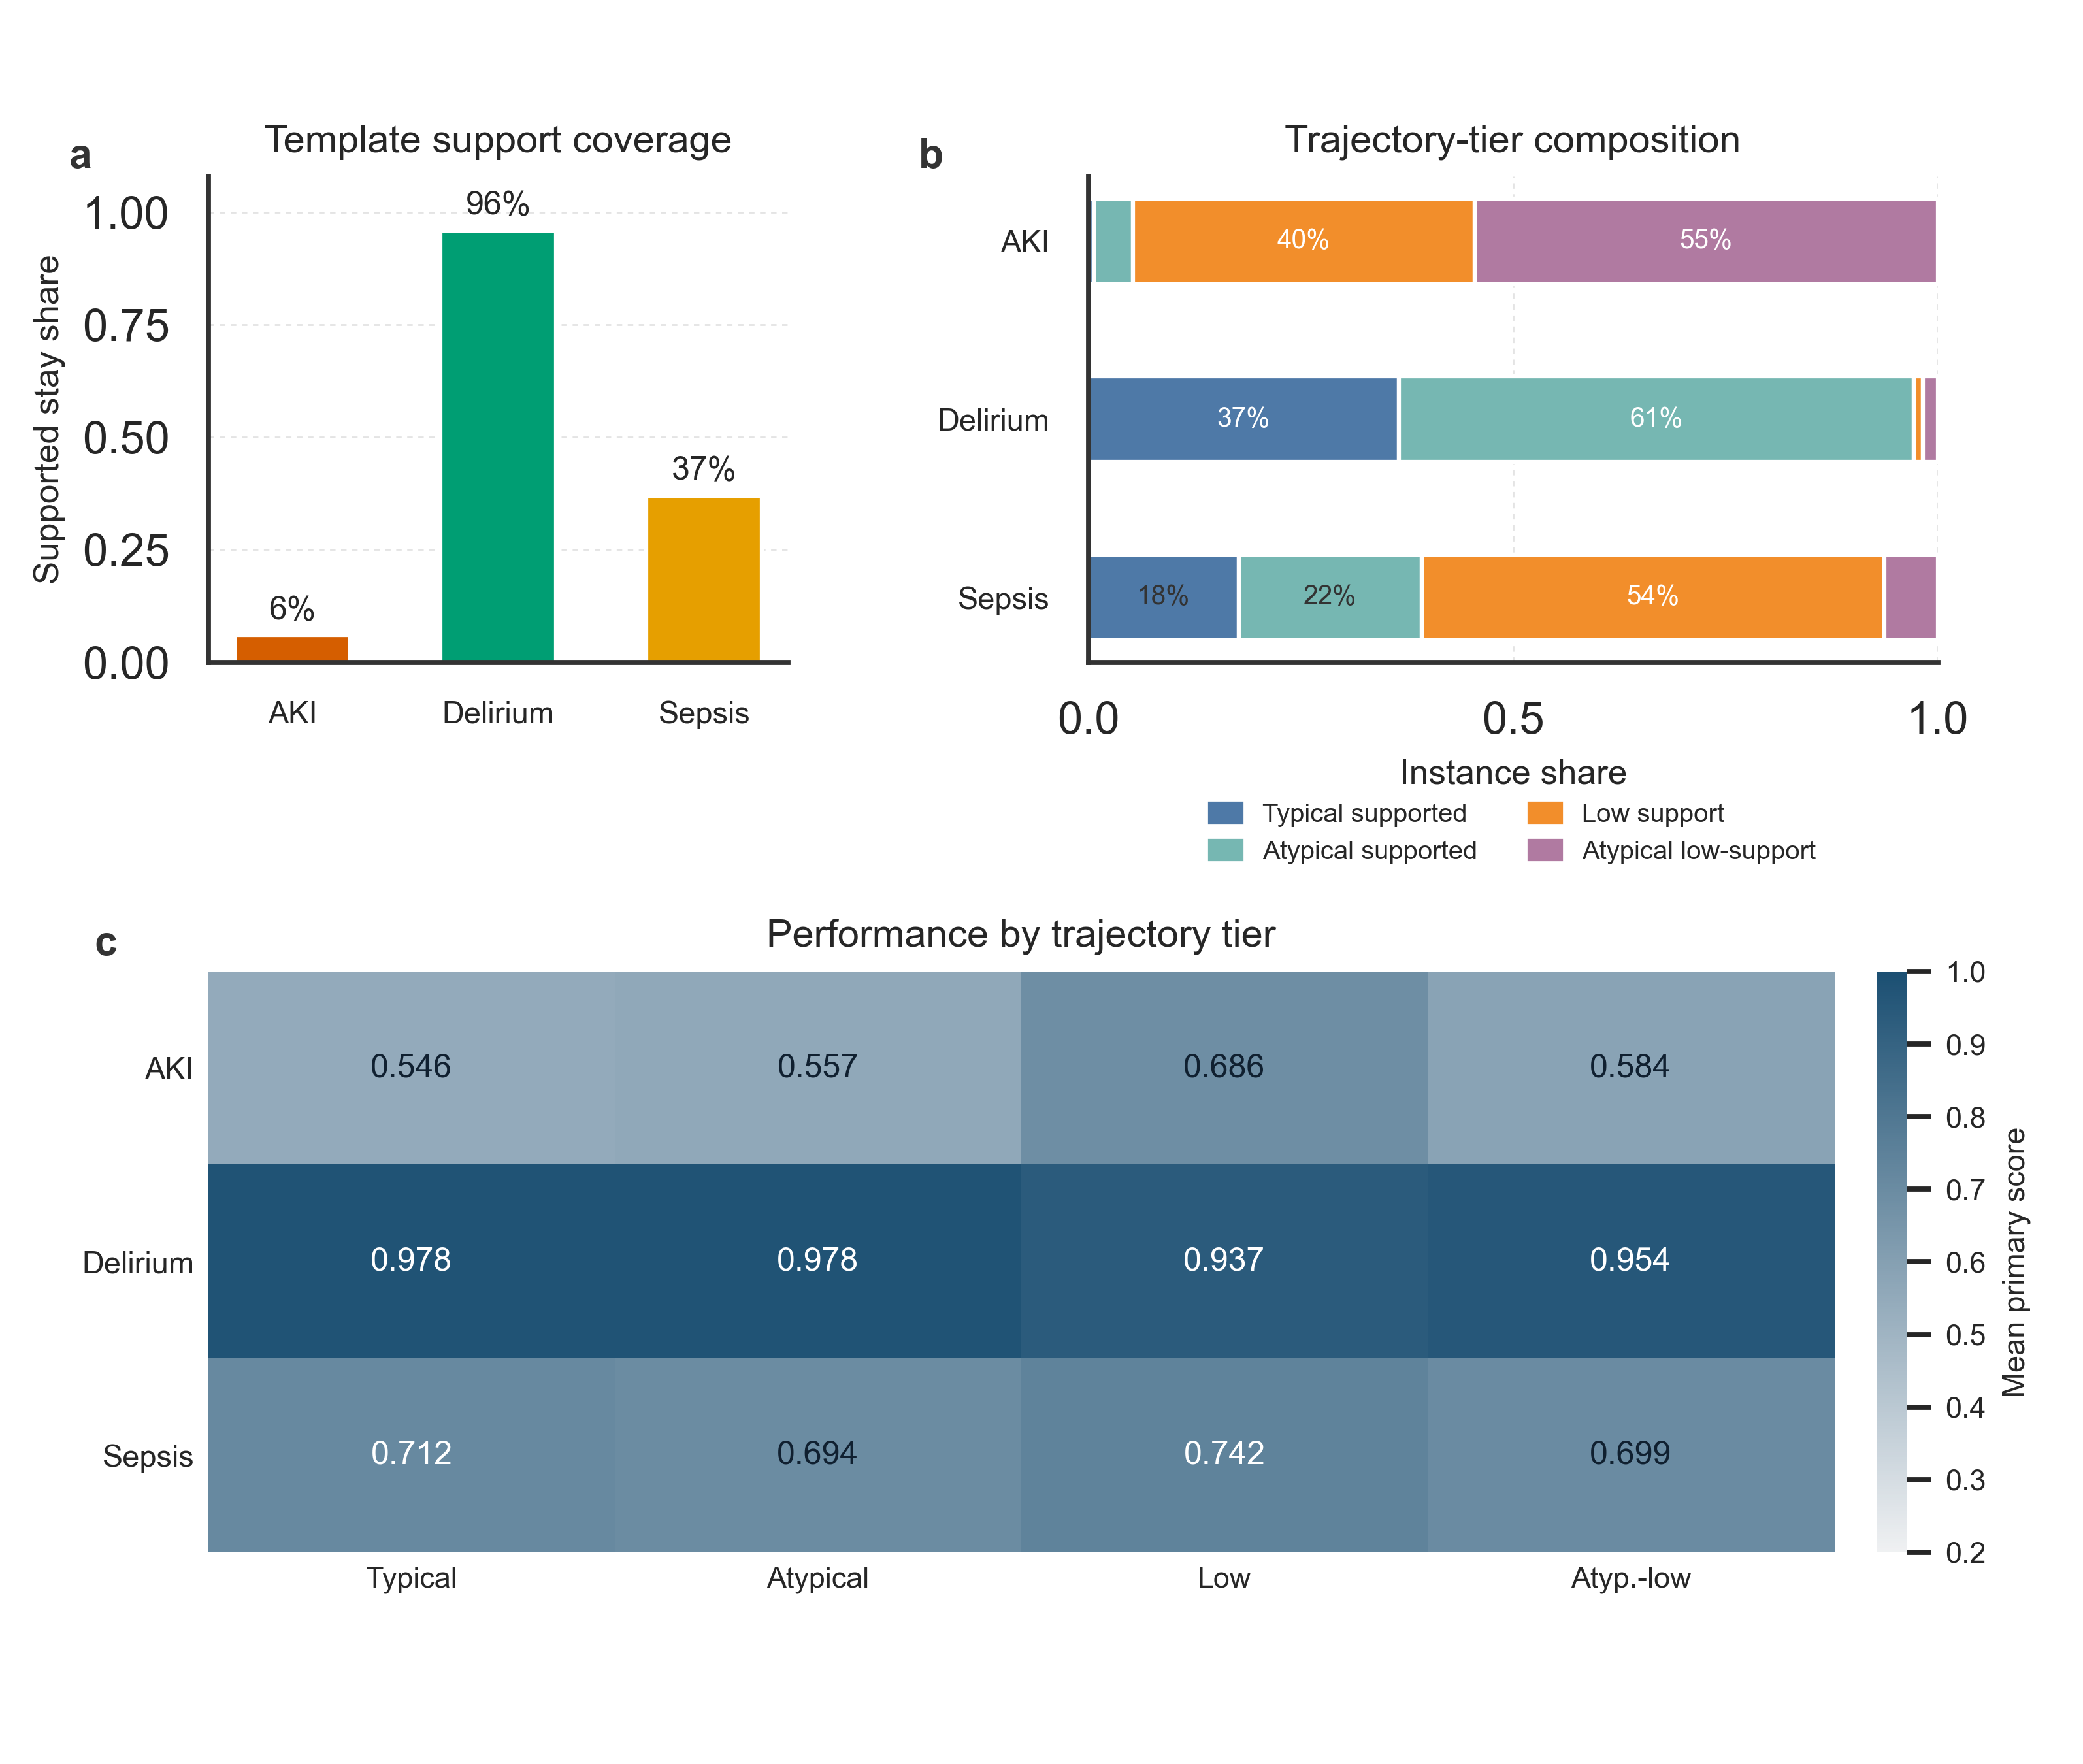
\includegraphics[width=\textwidth]{figures/main/figure6_template_state_space_stratification.png}
\caption{Template support revealed disease-specific trajectory regularity and exposed performance differences hidden in pooled averages. Panel a shows stay-level template support coverage for AKI, delirium, and sepsis. Panel b shows sample-instance composition across trajectory tiers; only major composition segments are labeled. Panel c shows row-level auto-scored mean primary score by trajectory tier. Template support is an evidence-support / templatability measure, not a model-performance metric. The higher score in the AKI low-support stratum likely reflects easier non-progression case mix rather than a universal benefit of low support.}
\label{fig:trajectory_tier}
\end{figure*}

\FloatBarrier

\subsection{Judge-based evaluation preserved the auto-scored provider ordering}

Judge evaluation tested whether the auto-scored ordering persisted on deferred and hard-disagreement cases. The fixed roster included GPT-5.4, DeepSeek Chat, Aloe-70B, and MedGemma-4B. The packet contained 500 prompt instances and 2,000 contestant responses, scored by Claude Opus 4.6, GPT-5.4, and Gemini 3.1 Pro on the same rows.

The judge summaries preserved the broad provider separation seen in auto-scoring (Table~\ref{tab:judge_provider_summary}; Fig.~\ref{fig:judge_provider_summary}). Scores were averaged across the three judges. GPT-5.4 led on all five rubric axes, followed by DeepSeek Chat, Aloe-70B, and MedGemma-4B. Cross-judge agreement was substantial: against Claude Opus 4.6, GPT-5.4 achieved Spearman $\rho$ 0.814 on overall quality and 0.808 on clinical correctness, while Gemini 3.1 Pro achieved 0.783 and 0.759. The judge phase therefore served as a structured complementary evaluation layer, not a substitute for human adjudication.

\begin{figure*}[t]
\centering
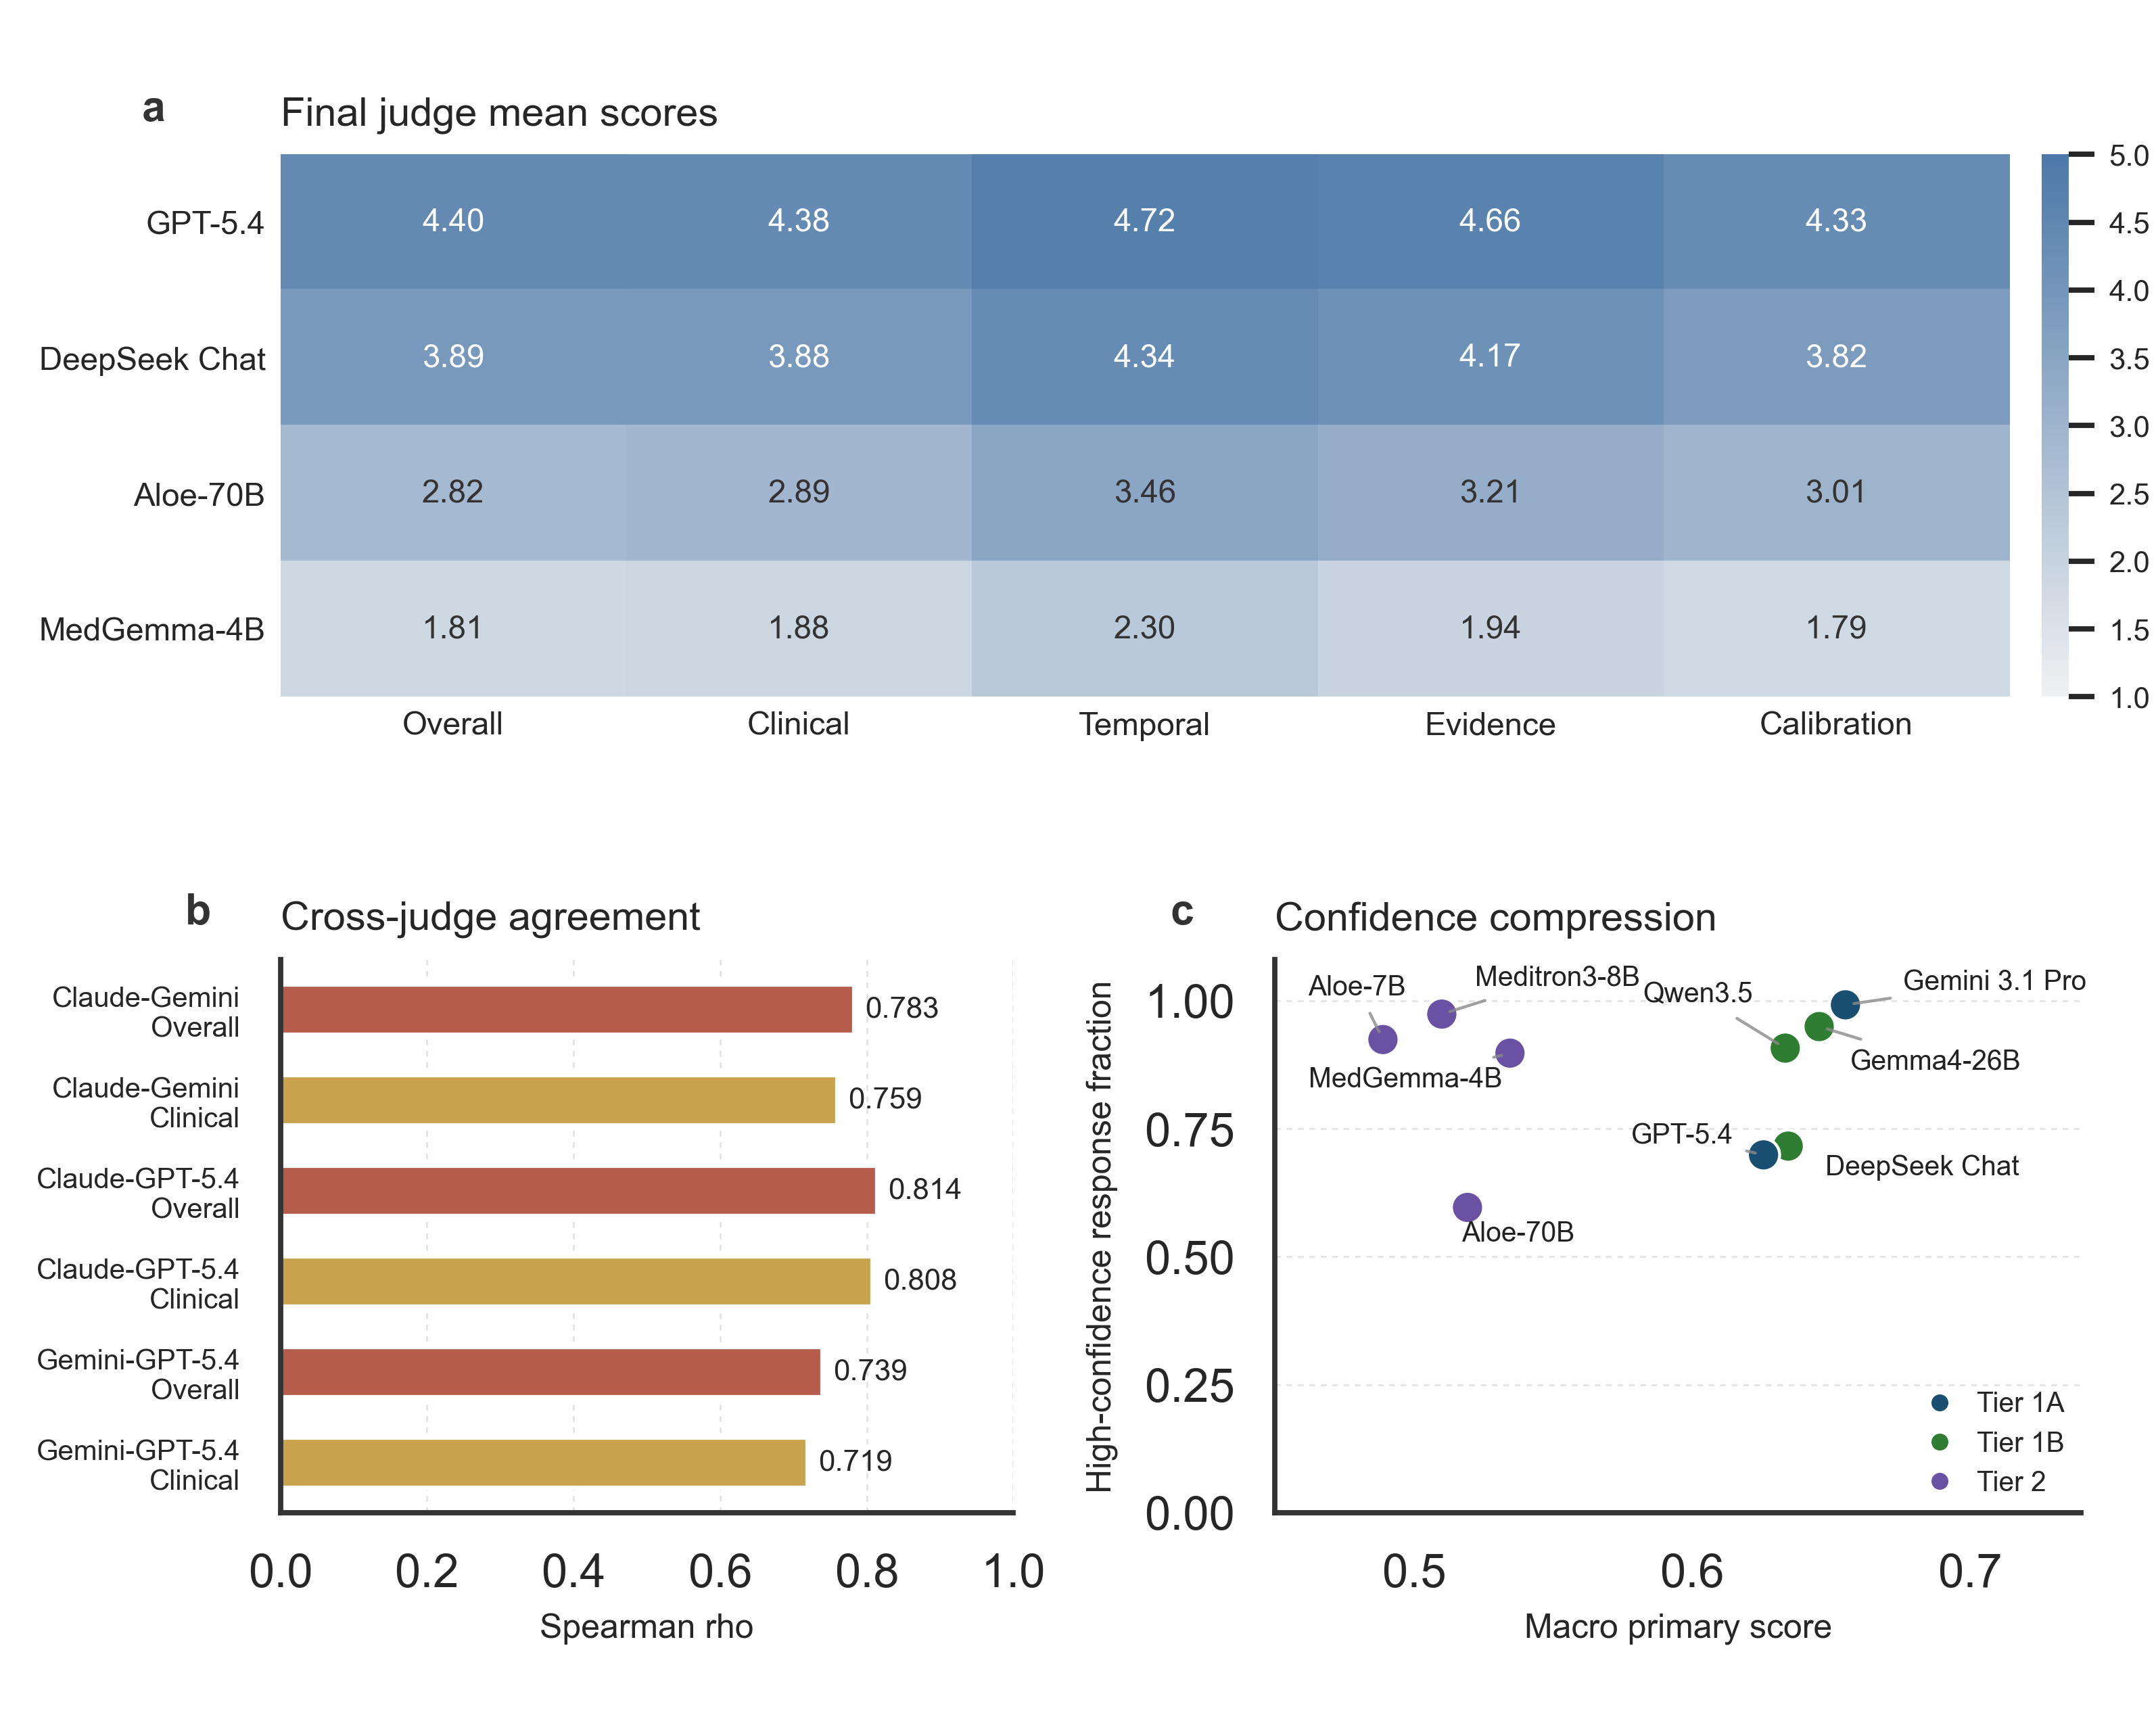
\includegraphics[width=\textwidth]{figures/main/figure7_judge_validation_calibration.png}
\caption{Judge-based evaluation preserved the broad provider ordering while revealing differences in response quality and confidence behavior. Panel a reports final mean scores across the three judges for overall quality, clinical correctness, temporal grounding, evidence grounding, and calibration for the four fixed judge-phase contestants. Panel b shows pairwise cross-judge Spearman correlations for overall quality and clinical correctness. Panel c compares overall macro primary score with the fraction of high-confidence responses across all nine providers; all provider points are labeled. Confidence fraction uses full 53,070-prompt provider summaries where available and is the share of parsed responses with \texttt{confidence\_value} equal to high, not statistical probability calibration. The judge packet contained 500 prompt instances and 2,000 contestant responses, evaluated by Claude Opus 4.6, GPT-5.4, and Gemini 3.1 Pro on the same rows.}
\label{fig:judge_provider_summary}
\end{figure*}

\begin{table*}[t]
\caption{Judge-based provider summary for the four fixed contestants, reporting mean rubric scores across the three judges on a 1--5 scale.}
\label{tab:judge_provider_summary}
\centering
\scriptsize
\begin{tabular}{@{}lrrrrr@{}}
\toprule
Provider & Overall & Clinical & Temporal & Evidence & Calibration \\
\midrule
GPT-5.4 & 4.397 & 4.383 & 4.722 & 4.655 & 4.325 \\
DeepSeek Chat & 3.894 & 3.882 & 4.342 & 4.167 & 3.819 \\
Aloe-70B & 2.823 & 2.885 & 3.464 & 3.209 & 3.008 \\
MedGemma-4B & 1.813 & 1.883 & 2.298 & 1.945 & 1.793 \\
\botrule
\end{tabular}
\normalsize
\end{table*}


\begin{table*}[t]
\caption{Judge agreement summary across the shared 2,000-row judge packet.}
\label{tab:judge_agreement}
\centering
\scriptsize
\begin{tabular}{@{}lllrrr@{}}
\toprule
Judge A & Judge B & Score & Rows & Spearman $\rho$ & Exact match rate \\
\midrule
Claude Opus 4.6 & Gemini 3.1 Pro & overall quality & 2000 & 0.783 & 0.283 \\
Claude Opus 4.6 & Gemini 3.1 Pro & clinical correctness & 2000 & 0.759 & 0.286 \\
Claude Opus 4.6 & GPT-5.4 & overall quality & 2000 & 0.814 & 0.527 \\
Claude Opus 4.6 & GPT-5.4 & clinical correctness & 2000 & 0.808 & 0.511 \\
Gemini 3.1 Pro & GPT-5.4 & overall quality & 2000 & 0.739 & 0.410 \\
Gemini 3.1 Pro & GPT-5.4 & clinical correctness & 2000 & 0.719 & 0.411 \\
\botrule
\end{tabular}
\normalsize
\end{table*}


\FloatBarrier

\section{Discussion}

Four findings stand out. Temporal clinical reasoning difficulty was strongly condition-dependent (RQ2): delirium was near ceiling, whereas stroke remained difficult. Explicit temporal sequence modeling did not uniformly outperform a compact structured summary (RQ1). General-purpose models led the aggregate comparison, while medical-domain models remained below Tier 1A and Tier 1B groups overall (RQ3). Finally, trajectory-template support carried information about reasoning difficulty and should be reported in temporal clinical benchmarks (RQ2).

The branch comparison challenges the assumption that more temporal detail is always beneficial. Branch B1 improved AUROC on only 3 of 7 eligible tasks and AUPRC on only 1 of 7. The defensible interpretation is narrower: temporal structure helps when it aligns with the task's decision boundary and is represented in a recoverable form. For other tasks, the anchor-state summary captured the relevant signal with less noise.

The aggregate tier gap is the most consequential benchmark-level result. All four Tier 2 medical-domain models underperformed the Tier 1A and Tier 1B groups in the aggregate macro comparison, although local condition-level rankings varied. This suggests that current medical adaptation is better aligned to medical language competence, knowledge recall, and static question answering than to anchor-bounded interpretation of evolving ICU evidence. The finding is consistent with broader clinical LLM evaluations showing that encoded medical knowledge does not automatically yield robust open-ended clinical decision making\cite{singhal2023clinicalknowledge,hager2024clinicaldecision}, and with calls for clinically relevant validation of generalist medical AI systems\cite{moor2023gmai,saab2024gemini}.

TIMELY Bench is complementary to existing benchmarks rather than a replacement for them. MedQA and PubMedQA test medical knowledge and biomedical reading comprehension\cite{jin2021medqa,jin2019pubmedqa}; HealthBench, MedHELM, and LLMEval-Med broaden open-ended clinical evaluation\cite{arora2025healthbench,bedi2025medhelm,zhang2025llmevalmed}; EHRSHOT evaluates few-shot transfer on coded longitudinal records\cite{wornow2023ehrshot}; and MedAgentBench tests interactive tool use in a virtual EHR environment\cite{jiang2025medagentbench}. TIMELY Bench goes deeper on a narrower construct: interpreting synchronized ICU evidence under a masked information boundary. That emphasis explains why medical-domain models such as Me-LLaMA and MEDITRON, designed to strengthen clinical language competence and medical task performance\cite{xie2025mellama,chen2023meditron}, did not necessarily outperform general-purpose models on this benchmark.

This distinction matters for how the results should be used. TIMELY Bench should not be read as a general ranking of medical usefulness, nor as evidence that domain-specific training is unnecessary. It shows that domain adaptation alone was insufficient for this particular composite skill: bounded longitudinal interpretation across structured data, notes, treatments, and condition-specific task definitions. Future domain adaptation may need to include longitudinal supervision, event-time objectives, and explicit evidence-grounding targets rather than only medical corpora or question-answering data.

CRES made the failure modes more interpretable. D3 trend reasoning was comparatively strong, D2 threshold reasoning separated tiers sharply, and D4 diagnostic discrimination was weak across the board. Current models can often detect directional change once the relevant signal is explicit, but struggle when the task requires selecting among overlapping clinical explanations. Confidence behavior also mattered. Gemini 3.1 Pro achieved the highest overall macro score but marked 99.2\% of prompts as high confidence, compared with 69.9\% for GPT-5.4. This is not statistical calibration, but it is relevant for deployment-facing evaluation because over-compressed confidence labels limit selective escalation and uncertainty-aware review.

The clinical significance of TIMELY Bench is not that it identifies a deployable model. It provides a pre-deployment evaluation scaffold for asking whether a model respects an ICU information boundary, recognizes threshold crossing, distinguishes atypical or low-support trajectories, and attributes its answer to visible evidence. This logic is relevant beyond the four conditions studied here. Trial recruitment, endpoint abstraction, pharmacovigilance, and rare disease natural-history work increasingly use longitudinal EHR data, and each depends on whether progression or safety events are identifiable from evidence available at the relevant time\cite{fda2023rwe,richesson2013ehrphenotyping,wang2009pharmacovigilance,harpaz2012adverseevent,fda2019rarediseasehistory,bastarache2018phers}. TIMELY Bench does not validate models for those operational uses, but it offers a testable structure for future disease-specific extensions.

In that sense, the benchmark is closer to a diagnostic instrument than to a deployment scorecard. It can reveal whether a candidate model fails because it ignores the temporal boundary, cannot map measurements to thresholds, overuses confidence labels, or lacks sufficient evidence grounding. Those distinctions are clinically meaningful because the mitigation differs in each case: better serialization, different supervision, human review, or exclusion from a particular workflow.

Trajectory-template support is a methodological contribution in its own right. Delirium, sepsis, and AKI differed not only in performance, but in how often stays could be mapped onto executable physiology templates. The gap between delirium (96\% stay-level support) and AKI (6\%) indicates that disease-specific temporal regularity is part of the benchmark construct. Future temporal clinical benchmarks should report both task distributions and how much of the trajectory space is clinically templatable.

Several limitations follow from the study design. TIMELY Bench is retrospective and derived from one source environment, so it does not establish transportability across institutions, documentation cultures, or EHR systems. Stroke bypasses the B3 template layer, so the four condition families are not perfectly symmetric at the latent-state level. Judge evaluation is model-based rather than human-adjudicated; LLM-as-judge methods remain a complement to, not a substitute for, expert review\cite{zheng2023judging,bedi2025medhelm}. Cross-condition causal pathways such as septic AKI and septic encephalopathy are not modeled. The delirium anchor relies on CAM-ICU assessments (item 228332), which may underrepresent hypoactive delirium. SOFA decomposition for sepsis currently covers four of six organ components; neurological and coagulation components should be added in future iterations. The benchmark also does not include prospective evaluation in live clinical workflows. Any future interventional use would require prospective protocols and reporting aligned with AI-specific guidance such as SPIRIT-AI and CONSORT-AI\cite{rivera2020spiritai,liu2020consortai}.

Taken together, these results support TIMELY Bench as a diagnostic instrument for temporal clinical AI evaluation. It frames temporal reasoning as a condition-aware, anchor-bounded, multi-representation problem, exposes when temporal structure helps and when it does not, and makes disease-specific trajectory support visible. That role is narrower than clinical deployment, but broader than a leaderboard.

\section{Methods}

\subsection{Study design and source data}

TIMELY Bench was constructed as a phase-locked benchmark for temporal clinical reasoning over ICU data derived from MIMIC-IV v3.1 and MIMIC-IV Note\cite{johnson2023mimic}. Source tables were accessed through the credentialed PhysioNet BigQuery distribution, including ICU, hospital, derived, discharge-note, and radiology-note modules. The pipeline aligned structured and textual evidence onto a 168-hour grid; built physiology templates for AKI, delirium, and sepsis; materialized synchronized representation branches; assembled condition-specific CRES tasks; reconstructed state-space trajectories; and froze the benchmark release for canonicalization, scoring, and comparison. The study is retrospective and methodologically aligned to STROBE, RECORD, and MI-CLAIM reporting domains\cite{vonelm2007strobe,benchimol2015record,norgeot2020miclaim}.

The benchmark was anchor-bounded by design. Each prompt instance corresponds to one stay, one task, one reasoning dimension, and one anchor hour. Evidence visible to the model is truncated to ICU admission through that anchor, and future information is masked. This prevents temporal reasoning from being conflated with retrospective leakage and allows the same stay to be evaluated under multiple information states.

The same anchor-bounded rule governs the prospective tasks in AKI, delirium, sepsis, and stroke Layer 1. Stroke Layer 2 is explicitly retrospective and is analyzed as a separate layer because mechanism, treatment strategy, NIHSS extraction, and complication labels depend on discharge or stay-level context. This separation avoids treating retrospective synthesis as if it were the same prediction problem as pre-anchor deterioration detection.

This study used de-identified data from MIMIC-IV v3.1 and MIMIC-IV Note, available through the PhysioNet credentialed data access program and its BigQuery-hosted release. Access requires completion of a recognized human subjects training course and signing of a data use agreement. The MIMIC-IV dataset was collected under a waiver of informed consent approved by the Beth Israel Deaconess Medical Center institutional review board. No additional ethical approval was required for this secondary analysis of de-identified data. This study did not involve any prospective data collection, patient contact, or intervention.

\subsection{Hourly alignment and synchronized representations}

Heterogeneous EHR sources were mapped to hourly or event-time representations over the first 168 ICU hours, including structured observations, medications, procedures, diagnosis-pathway events, and note fragments. Four synchronized views were then materialized for the same stay and anchor. Branch A is a compact structured summary for conventional baselines. Branch B1 preserves an explicit hourly sequence. Branch B2 is the prompt-ready multimodal EHR representation used for LLM evaluation; here, multimodal means EHR modalities, not imaging or audio. Branch B3 reconstructs a low-dimensional state-space trajectory for AKI, delirium, and sepsis.

The Phase 5 template layer applied condition-specific executable rules derived from physiology templates rather than inferring latent mechanisms from free text. These rules converted B3 trajectories into coarse phase labels and trajectory tiers using template-defined phase windows, expected marker trajectories, and atypical variants. Template support scores quantify observation coverage within phase-aligned windows; they do not prove that the full clinical narrative follows an idealized trajectory.

This distinction matters because template support is a data-availability and templatability measure, not a hidden label of disease truth. A low-support stay can still be clinically valid; it simply lacks enough aligned observations for the executable template to assign a high-confidence phase pattern.

\subsection{Condition definitions and label construction}

\noindent\textbf{AKI.} AKI construction used the derived \texttt{kdigo\_stages} table and retained stays with AKI evidence. Onset was anchored to the first hour meeting KDIGO Stage 1 criteria: creatinine increase of at least 0.3 mg/dL within 48 hours, creatinine at least 1.5 times baseline, or urine output below 0.5 mL/kg/h for at least 6 hours\cite{kdigo2012aki}. Stage 1, Stage 2+, Stage 3, and renal replacement therapy (RRT) proxy timing were extracted from derived tables, procedure events, and hourly RRT indicators. Anchors were emitted every 4 hours after Stage 1 onset. AKI-T1 is positive if Stage 2+ onset falls in $(T, T+24]$; AKI-S1 is positive if an RRT proxy event falls in $(T, T+72]$. Post-progression anchors were excluded so prompts remained pre-escalation information states.

\noindent\textbf{Delirium.} Delirium onset was anchored to the first positive CAM-ICU assessment from charted delirium assessments (itemid 228332), requiring the patient to be assessable at RASS $\geq -3$\cite{ely2001camicu}. The template approximated DSM-5 delirium constructs using executable hourly ICU observations rather than bedside neuropsychiatric narratives\cite{apa2013dsm5}. DEL-T1 captures persistent delirium within $(T, T+24]$; DEL-S1 captures resolution within $(T, T+24]$ using a sustained 24-hour non-positive window. Labels retain \texttt{left\_censored}, delirium-hour counts, and support flags for RASS, GCS, and restraints to separate physiology from observation sparsity.

The delirium label is therefore a structured screening-derived proxy, not an expert chart-adjudicated psychiatric diagnosis. Retaining left-censoring and support fields was necessary because delirium can be present before the first observable assessment and because sedation can make screening uninterpretable.

\noindent\textbf{Sepsis.} Sepsis construction started from stays flagged \texttt{sepsis3} and derived onset timing from diagnosis-pathway events. Explicit sepsis-onset events defined the onset hour when available; otherwise onset was set to hour zero and marked \texttt{onset\_confidence=low}. Septic shock was operationalized as mean arterial pressure below 65 mmHg with active vasopressor support, with lactate $>2$ mmol/L as an additional gate when available, consistent with Sepsis-3 and Surviving Sepsis Campaign guidance\cite{singer2016sepsis3,evans2021surviving}. Anchors were emitted every 4 hours after sepsis onset. SEP-T1 is positive when first post-onset shock falls in $(T, T+12]$; SEP-S1 is positive when lactate in $(T, T+6]$ falls to at most 90\% of observed baseline. Metadata records lactate, vasopressor, and SOFA support because many sepsis failures reflect support availability rather than reasoning alone.

Sepsis tasks were therefore designed around deterioration after a sepsis information state, not around discovering sepsis de novo from the entire record. The \texttt{onset\_confidence} field allows analyses to separate high-confidence onset timing from low-confidence pathway-derived defaults.

\noindent\textbf{Stroke.} Stroke used a stricter phenotype filter: only stays with \texttt{stroke\_subtype\_priority == "ischaemic"} entered the main benchmark, consistent with acute ischaemic stroke pathways\cite{berge2021eso}. Layer 1 contains anchor-bounded temporal tasks over motor strength, affected side, imaging consistency, and sequence signatures. S-T1 asks whether limb strength worsens in the next 12 hours; S-T2 derives affected side; S-T3 compares neurological laterality with first brain imaging; and S-T4 summarizes the temporal ordering of assessment, pathway activation, imaging, and first worsening. Layer 2 contains retrospective mechanism, strategy, NIHSS extraction, and complication tasks from discharge summaries and stay-level context. Eligibility was defined from data coverage tiers: Layer 1 required sufficiently dense neurological observations, whereas Layer 2 required retrospective summary content.

This two-layer design was retained because stroke combines short-horizon neurological evolution with retrospective clinical synthesis. Pooling the two would make stroke appear artificially inconsistent: the same condition contains both prediction tasks under future masking and tasks that intentionally use the full documented course.

\subsection{Prompt serialization and evaluation variants}

The formal LLM evaluation used Branch B2 and a fixed ``Modality-Separated Sections'' serialization. Prompts begin with a system instruction and patient-context header naming the condition, task, and anchor hour, followed by sections for demographics, structured hourly timeline, medications, procedures, and clinical notes; stroke temporal prompts additionally include neurological assessments. Hour markers are preserved in the canonical \texttt{full\_multimodal} variant. Each prompt ends with a task-specific question and a fixed JSON schema containing \texttt{reasoning}, \texttt{answer}, timestamped \texttt{evidence}, and \texttt{confidence}.

Five variants were materialized: \texttt{full\_multimodal}, \texttt{structured\_only}, \texttt{text\_only}, \texttt{no\_temporal\_markers}, and \texttt{shuffled\_timeline}. Formal comparative results use only the frozen \texttt{full\_multimodal} variant. Structured baselines were evaluated only on eligible binary tasks. Branch A used XGBoost on 384 engineered anchor-state features. Branch B1 used BiLSTM-attention and temporal-transformer models on fixed-length 168-hour structured sequences aligned to the same anchor-bounded evidence state. Missingness was represented by released masks and eligibility fields, and all baselines used five-fold subject-level cross-validation. Figure~\ref{fig:branch_comparison} uses the B1 model selected by AUROC within each task as the shared B1 comparator for both AUROC and AUPRC deltas.

Prompt serialization was deterministic. If a value was absent from a rendered hour, it means the value was not available in that hour's visible evidence stream, not that it was imputed as normal or zero. This convention preserves the distinction between physiologic absence, measurement absence, and post-anchor masking.

\subsection{CRES dimensions and operational scoring}

The Clinical Reasoning Evaluation Suite (CRES) decomposes temporal clinical reasoning into six dimensions. D1 temporal localization asks when the earliest sign of the target event became visible. D2 threshold reasoning asks whether a clinically meaningful threshold was crossed and, if so, when. D3 trend interpretation asks whether the relevant signal is improving, stable, or worsening. D4 diagnostic discrimination asks which explanation or mechanistic category best fits the evidence. D5 contrastive reasoning asks the model to choose between competing trajectory types or support classes, such as typical versus atypical or high-confidence versus low-confidence onset. D6 attribution asks the model to identify the evidence items that most strongly support the answer.

Operationalization is task-specific rather than one-size-fits-all. For example, AKI-T1 D1 and D2 are event-time tasks keyed to Stage 2+ onset, stroke S-T1 D3 is a binary trend task keyed to future strength worsening, stroke S-R3 D2 is a numeric-exact extraction task keyed to NIHSS peak, and sepsis SEP-T1 D5 is a categorical contrastive task keyed to onset-confidence class. The generalized auto-scoring pipeline reused the same parser, truth builder, and scoring rules originally validated on Tier 1A. Primary score was defined as binary accuracy for event-time and binary tasks, macro F1 for categorical tasks, and exact match for numeric extraction. Provider-level macro primary score was computed as the equal-weight mean of the 20 supported task-dimension primary scores for each provider, not as a row-weighted mean. Condition-level and CRES-dimension summaries used the same equal-weight macro aggregation within the relevant condition or dimension subset. D6 remained deferred from the primary auto-scoring pipeline and was instead assessed in the judge phase.

For event-time tasks, the scorer first normalizes abstentions, no-event answers, and explicit hour values before comparing them with the task truth object. Thus an answer can be correct either by identifying the correct event state or by correctly abstaining when the visible anchor-bounded evidence does not support an event within the target horizon. This matters for examples such as AKI-T1 D1, where overcalling a plausible but unsupported hour is treated as a temporal localization error.

Formal auto-scoring covered 20 supported task-dimension pairs and deferred 27 pairs. Because dimension coverage is not uniform across tasks, per-dimension summaries should be interpreted as structured slices of the benchmark rather than as interchangeable skill estimates. This is especially important for D3 and D4, which are dominated by stroke tasks, and D5, which is concentrated in AKI and sepsis contrastive prompts.

\begin{table*}[t]
\caption{Operational definition of the six Clinical Reasoning Evaluation Suite (CRES) dimensions. Supported auto-scored pairs are evaluated in Phase 6.5F; D6 attribution remains judge-deferred in the primary results.}
\label{tab:cres_dimensions}
\centering
\small
\setlength{\tabcolsep}{4pt}
\begin{tabularx}{\textwidth}{>{\raggedright\arraybackslash}p{0.09\textwidth} >{\raggedright\arraybackslash}p{0.25\textwidth} >{\raggedright\arraybackslash}X >{\raggedright\arraybackslash}p{0.15\textwidth} >{\raggedright\arraybackslash}p{0.12\textwidth}}
\toprule
Dimension & Clinical question type & Truth construction in TIMELY Bench & Primary score & Formal status \\
\midrule
D1 Temporal localization & When did the earliest sign of the target event become visible? & Earliest post-anchor onset hour from task tables, such as Stage 2+ onset, delirium onset, sepsis onset, or first neurological worsening hour. & Binary accuracy on event-time detection & Auto-scored \\
D2 Threshold reasoning & Has a clinically meaningful threshold been crossed, and if so when? & Guideline-linked or task-linked threshold hour, such as KDIGO stage crossing, RRT proxy timing, septic shock onset, or peak NIHSS value. & Binary accuracy or exact match, depending on task & Auto-scored \\
D3 Trend interpretation & Is the relevant physiological signal improving, stable, or worsening? & Future trajectory label derived from structured follow-up windows, most prominently stroke motor-strength worsening and related temporal tasks. & Binary accuracy & Auto-scored where supported \\
D4 Diagnostic discrimination & Which clinical explanation best fits the observed evidence? & Categorical truth from stay-level labels such as affected side, imaging-consistency class, stroke mechanism, treatment strategy, or complication presence. & Macro F1 & Auto-scored \\
D5 Contrastive reasoning & Which competing trajectory archetype best matches the case? & Condition-specific contrast labels, including AKI typical versus atypical trajectory class and sepsis onset-confidence class. & Macro F1 & Auto-scored where supported \\
D6 Attribution & Which evidence items most strongly support the answer? & Judge-facing evidence grounding over the submitted timestamped evidence triples and free-text rationale. & Rubric-based judge scoring & Deferred from primary auto-scoring \\
\bottomrule
\end{tabularx}
\end{table*}


\subsection{Illustrative prompt instance and response contrast}

Box 1 illustrates the serialization using an AKI-T1 D1 instance at anchor hour 11. This is a negative example because no AKI Stage 2+ onset occurs within the 24-hour horizon after the anchor. GPT-5.4 correctly abstains from assigning an onset hour, whereas MedGemma-4B overcalls Hour 4 from transient hypotension, showing how plausible physiology narratives can diverge from the benchmark target. Displayed prompt lines are copied from the frozen prompt, with whole blocks omitted only between explicit truncation markers.

\begin{center}
\footnotesize
\setlength{\fboxsep}{5pt}
\textbf{Box 1 | Illustrative TIMELY Bench prompt instance and model responses.}\par
\vspace{4pt}
\begin{minipage}[t]{0.48\textwidth}
\textbf{Prompt structure (AKI-T1, D1, anchor = Hour 11)}\par
\vspace{4pt}
\fbox{\parbox[t]{0.96\linewidth}{\ttfamily\scriptsize\raggedright
{[SYSTEM]}\\
Reason step by step, cite measurements and timestamps, and answer based ONLY on the data provided.\\[3pt]
{[PATIENT CONTEXT]}\\
=== PATIENT CONTEXT (Condition: aki, Task: AKI-T1, Anchor: Hour 11.0) ===\\[3pt]
=== SECTION 1: DEMOGRAPHICS \& COMORBIDITIES ===\\
62-year-old M. ckd.\\[3pt]
=== SECTION 2: STRUCTURED TIMELINE ===\\
{[Hour 0]} map\_merged=92.0; spo2=98.0; sofa\_total=0\\
{[Hour 1]} heart\_rate=82.0; map\_merged=79.0; spo2=100.0; rrt\_active=1; sofa\_total=0\\
{[Hour 4]} heart\_rate=73.0; map\_merged=62.0; spo2=100.0; rrt\_active=1; sofa\_total=1\\
{[Hour 7]} heart\_rate=81.0; map\_merged=121.0; spo2=99.0; urineoutput\_hourly=200.0; rrt\_active=1; sofa\_total=1\\
\ldots{} truncated; prompt continues through Hour 11 \ldots\\[3pt]
=== SECTION 3: MEDICATIONS ===\\
No events in window.\\[3pt]
=== SECTION 4: PROCEDURES ===\\
No events in window.\\[3pt]
=== SECTION 5: CLINICAL NOTES ===\\
{[Hour 0]} {[nursing]} Patient Verbalized\\
\ldots{} truncated; prompt contains additional nursing lines through Hour 9 \ldots\\[3pt]
{[QUESTION]}\\
At what hour did the earliest sign of AKI Stage 2 progression appear?\\[3pt]
{[FORMAT]}\\
\{reasoning, answer, evidence[], confidence\}
}}
\end{minipage}\hfill
\begin{minipage}[t]{0.49\textwidth}
\textbf{Strong response (GPT-5.4; correct)}\par
\vspace{4pt}
\fbox{\parbox[t]{0.96\linewidth}{\ttfamily\scriptsize\raggedright
"reasoning": "Stage 2 progression would require creatinine worsening or sustained oliguria. No creatinine values are visible, urine output is preserved, and RRT is already active from Hour 1; therefore the window contains no new identifiable Stage 2 signal."\\
"answer": "No clear hour identified."\\
"evidence": [\\
\hspace*{1em}\{"timestamp":"Hour 1","measurement":"rrt\_active","value":"1"\},\\
\hspace*{1em}\{"timestamp":"Hour 7","measurement":"urine output","value":"200 mL"\}\\
]\\
"confidence": "low"
}}\par
\vspace{8pt}
\textbf{Weak response (MedGemma-4B; incorrect)}\par
\vspace{4pt}
\fbox{\parbox[t]{0.96\linewidth}{\ttfamily\scriptsize\raggedright
"reasoning": "MAP fell from 93 to 62 by Hour 4, suggesting worsening renal perfusion and AKI progression."\\
"answer": "Hour 4"\\
"evidence": [\{"timestamp":"Hour 4","measurement":"MAP","value":"62"\}]\\
"confidence": "high"
}}
\end{minipage}
\par\vspace{4pt}
\parbox{0.96\textwidth}{\footnotesize The example uses a frozen AKI-T1 D1 prompt from the formal evaluation packet and contrasts a strong temporal localization response with a weak one on the same anchor-bounded evidence state. All displayed prompt lines are verbatim from the frozen prompt; truncation is applied only between blocks for space. Full \texttt{full\_multimodal} prompts averaged approximately 1,978 tokens in the frozen 12k evaluation sample. For this instance, the correct benchmark label is that no AKI Stage 2+ onset is identifiable within the 24-hour prediction horizon after the anchor.}
\end{center}

\subsection{Frozen evaluation sample, contestant set, and canonicalization}

The frozen evaluation sample contained 12,000 benchmark instances from 9,587 ICU stays. Sampling was stratified by task and condition and capped at two anchors per stay per task, except for stay-level stroke tasks. Expanding this sample across the supported task-dimension map yielded 53,070 \texttt{full\_multimodal} prompt rows per provider.

The frozen comparative set contained nine providers: GPT-5.4, Gemini 3.1 Pro, DeepSeek Chat, Qwen3.5, Gemma4-26B, Aloe-70B, Aloe-7B, Meditron3-8B, and MedGemma-4B. Tier 1A denoted closed general-purpose API models, Tier 1B general-purpose open or semi-open models, and Tier 2 medical-domain adapted models. OpenBioLLM-70B was excluded from formal comparison because its effective context ceiling was not adequate for the released prompt format and was replaced by Aloe-70B. The original Me-LLaMA slot was replaced by Aloe-7B before comparative scoring.

Canonicalization required one response file per provider with 53,070 unique prompt identifiers, \texttt{status=ok}, and \texttt{parse\_success=true}. Aloe-70B, Aloe-7B, Meditron3-8B, and MedGemma-4B required audited overlay repair chains. For MedGemma-4B, 685 rows were overlaid through a vLLM repair path using the same frozen prompts, JSON schema, and parser. Provider-specific decoding defaults, output-token limits, and repair limits were not assumed identical; release manifests record provenance, row counts, token totals, latency summaries, and repair status. OpenBioLLM-70B was retained only as a supplementary artifact. Release manifests and scoring summaries were retained as documentation artifacts, following the principle that dataset consumers need explicit provenance and intended-use documentation\cite{gebru2021datasheets}.

\subsection{Auto-scoring, stratification, and judge evaluation}

The generalized Phase 6.5F scorer operated on the frozen provider registry, 12k evaluation sample, and Branch B2 prompt manifest. A parity check confirmed that GPT-5.4 and Gemini 3.1 Pro outputs matched the original Tier 1A supported task-dimension results up to floating-point rounding. Comparative outputs included provider tables, condition heatmaps, temporal degradation summaries, and stratified analyses by trajectory tier and stroke layer. Temporal degradation used predefined buckets: T6 for anchor hours 4--8, T24 for 18--30, and T48 for 46--50; cells with fewer than 25 instances were marked as insufficient support.

Judge evaluation was built after the auto-scored comparative set froze. The packet contained 500 prompt instances, sampled as 125 per condition, with 60\% from deferred pairs and 40\% from hard auto-scorable disagreements. The fixed contestant roster was GPT-5.4, DeepSeek Chat, Aloe-70B, and MedGemma-4B, yielding 2,000 judged responses. Claude Opus 4.6 served as primary judge, with GPT-5.4 and Gemini 3.1 Pro as cross-check judges scoring the same packet, following general LLM-as-judge methodology adapted to structured clinical reasoning\cite{zheng2023judging}. CREATE was used to construct frozen scoring artifacts and the judge packet; final external judge execution, repair, and aggregation were completed in the synchronized local analysis workspace after the CREATE-side Claude API run was blocked by a provider-side Cloudflare response.

\section*{Data availability}

The source clinical data used in this study are available through the PhysioNet credentialed data access program and BigQuery-hosted MIMIC-IV v3.1 and MIMIC-IV Note releases (MIMIC-IV, \url{https://physionet.org/content/mimiciv/}). Derived benchmark artifacts, including task manifests, evaluation samples, and scoring outputs, will be released upon publication.

\section*{Code availability}

The benchmark assembly, prompt serialization, and scoring code will be released in a public repository upon publication.

\section*{Acknowledgements}

The authors acknowledge the MIMIC-IV and PhysioNet teams for maintaining the de-identified critical care resource used in this study.

\section*{Author contributions}

H.W., Z.L., L.Q., and Z.I. contributed equally to the conception and design of the study, benchmark development, analysis and interpretation of results, figure design, and manuscript drafting and revision. All authors reviewed and approved the final manuscript.

\section*{Competing interests}

The authors declare no competing interests.

\bibliography{timely_bench_refs}

\end{document}
